%!TEX program=xelatex
\documentclass[chapter,book,openany,twoside]{oblivoir}
\usepackage{KNUworkshop2013,memtikzpagenodes}
\usepackage{tabu,subfig}
   \usepackage[dbl4x6]{fapapersize}
\usepackage[utf8]{inputenc} 
\begin{document}
%\displayPageLayout
\pagestyle{empty}
\title{참으로 멋진 인생 살았습니다 \\{\large 어공에서 늘공으로 그리고 전업농으로의 회귀}}
%\subtitle{(부제 : )}
\author{연천군청 지방공업주사 허호강}


\maketitle

\begin{figure}[h]
\centering 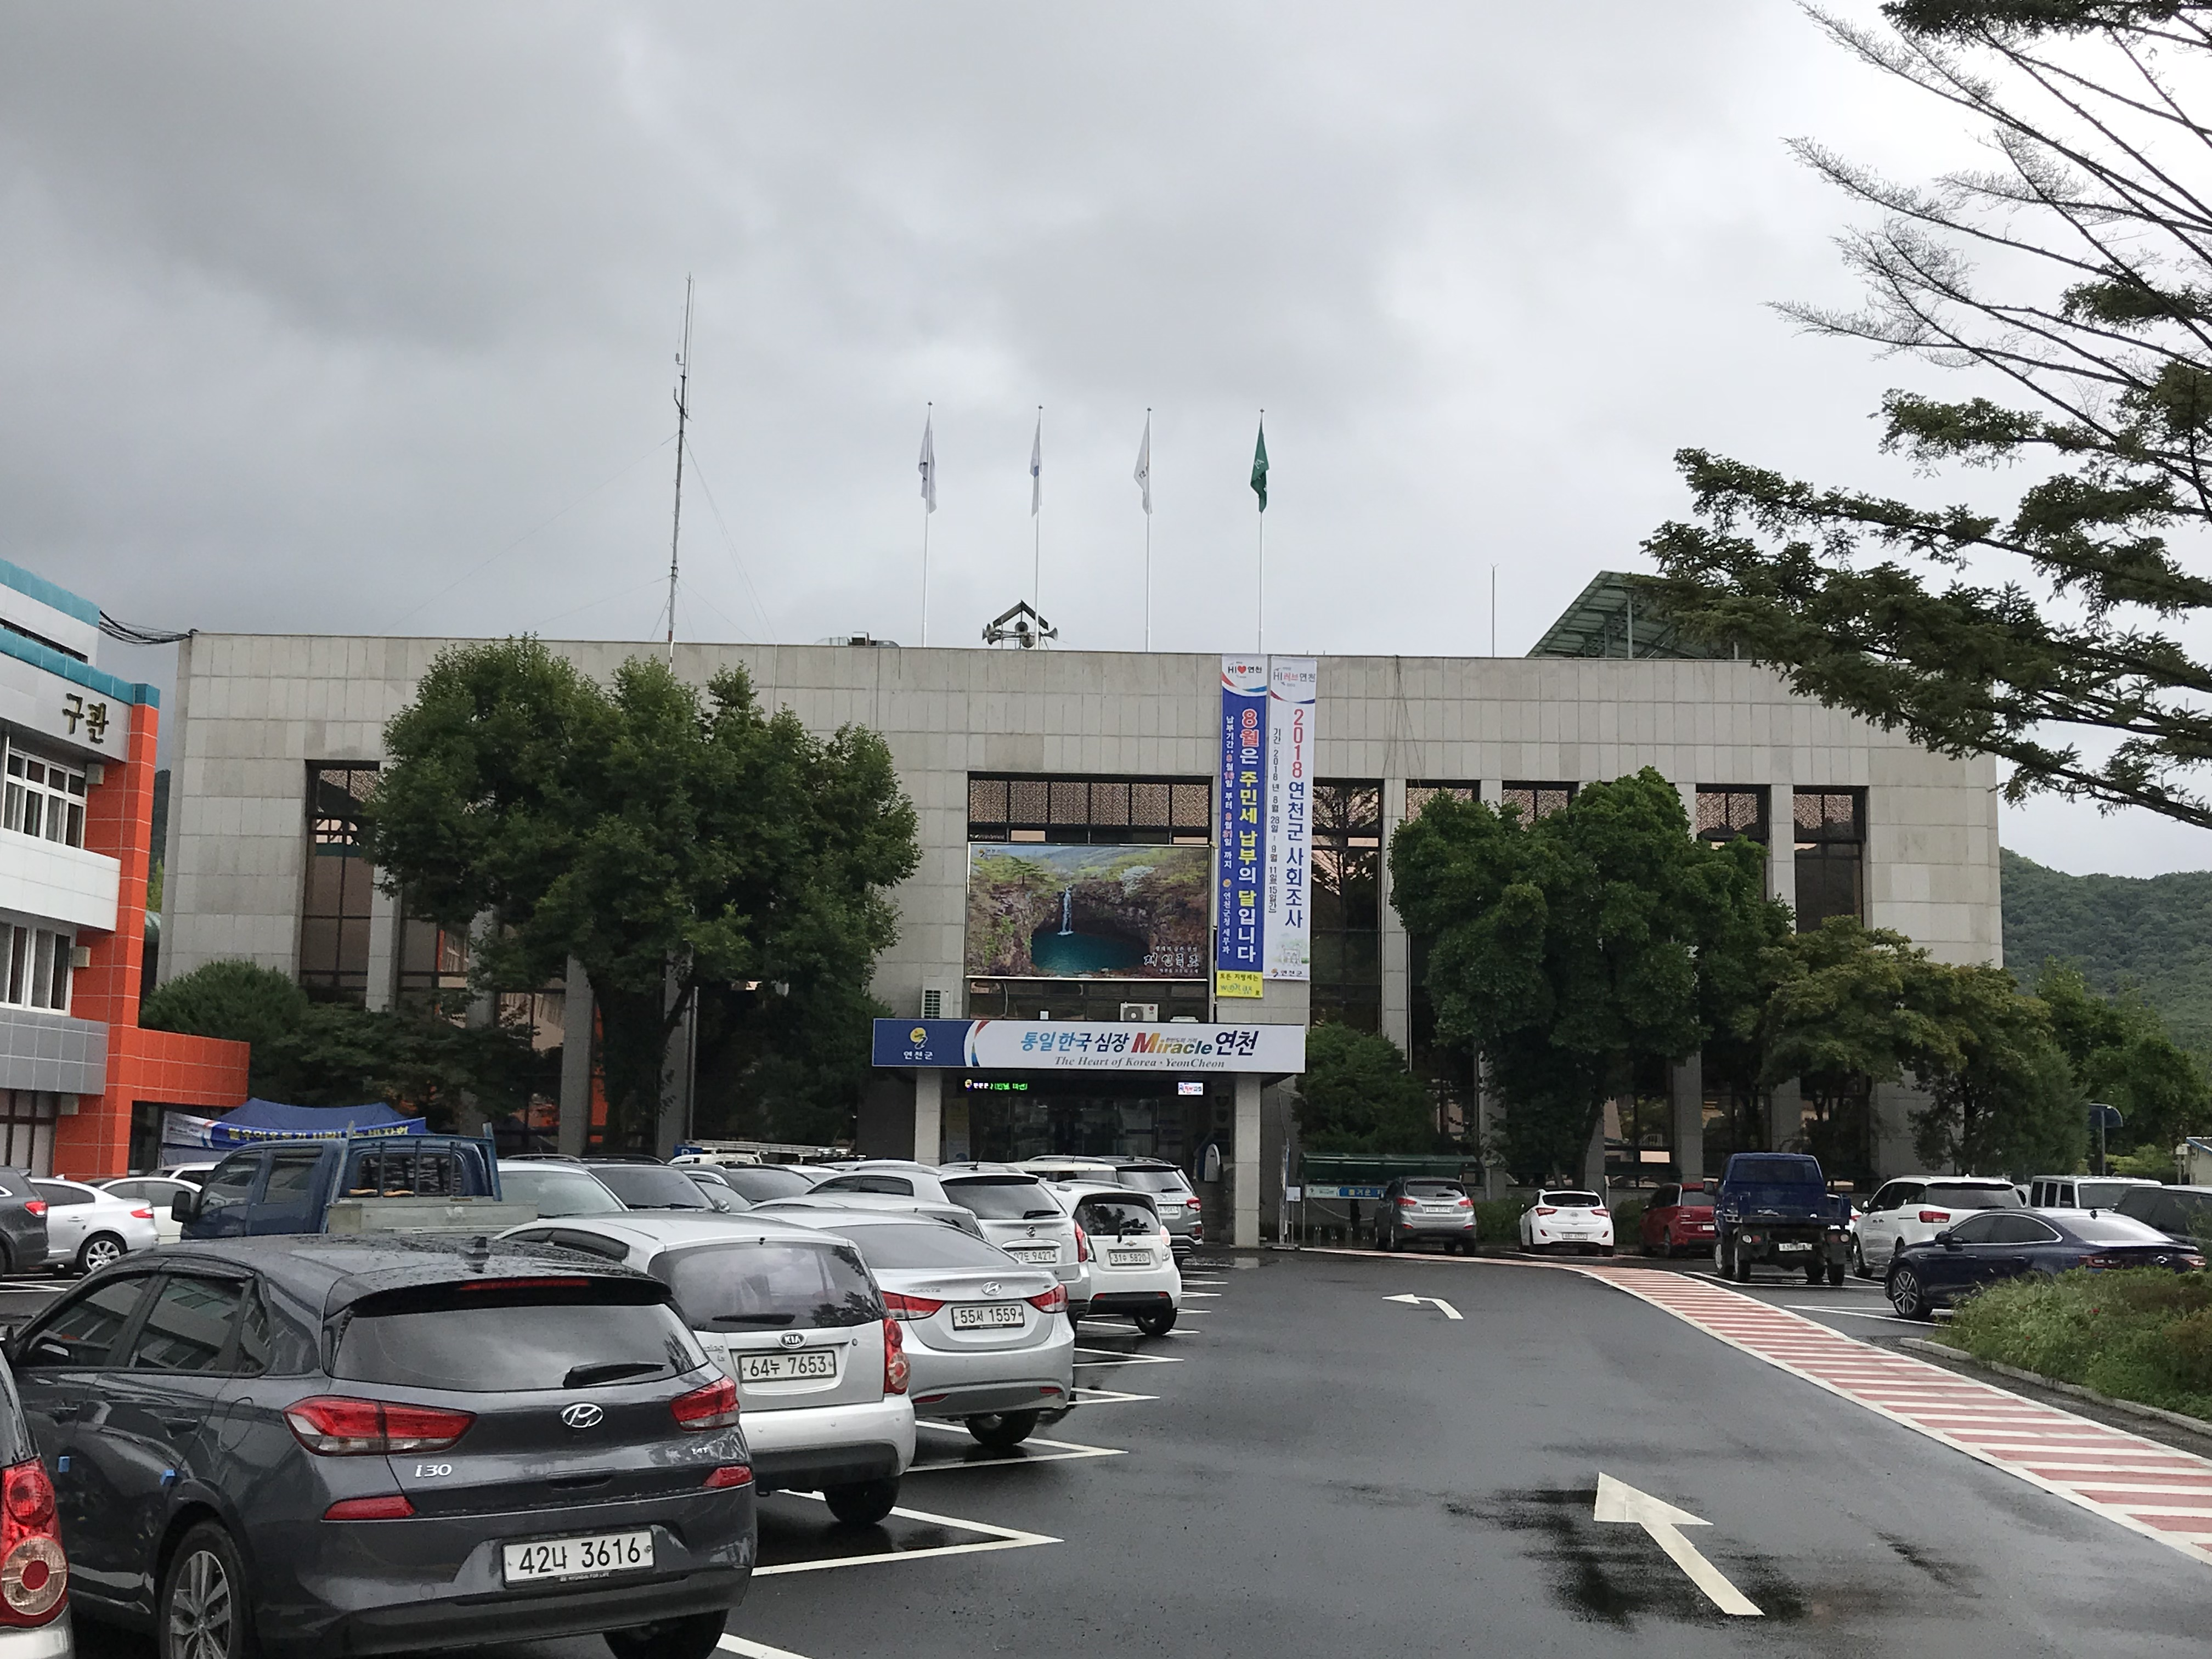
\includegraphics[scale=0.08]{DBs/pic/001.jpg}\\
\caption{30여년을 몸담았던 연천군청 전경}
\end{figure}
\newpage
\chapterstyle{KNUchapter}
\pagestyle{KNUworkshop}

\chapter{들어가기에 앞서}

저는 일반인으로서는 거의 평범하지 아니한 독특한 삶을 살아왔기에 그동안 제가 거쳐 온 지난날을 회상하며 저와 같이 희로애락을 느껴온 선후배 동료들에게 이러한 일들도 있었구나 하는 것을 남기고자 이 글을 씁니다.

저는 학창시절부터 목표가 공무원은 아니었습니다. 그때 당시의 저희 집에서는 아버지는 농업에 종사하시고 큰형은 1972년경 부터 자전거포로 시작하여 오토바이 수리점을 운영하고 계셨습니다.

아버지 또한 일제 강점기에 전기공사를 하는 전공을 하시고 6.25때에는 기갑부대에서 군복무를 하시다 상사로 전역 후 서울의 신촌에서 어머니의 반대를 무릅쓰고 지금의 대광리로 이사를 와서 방앗간을 운영하시는 큰집(아버님의 형님)에서 일을 하시다가 정미기 벨트에 감겨서 다치는 바람에 지금의 집으로 정착, 제가 태어나는 해인 1959년도부터 강냉이기계를 가지고 뻥튀기와 함께 기름도 짜고 국수를 만들어 파는 일을 하시면서 발동기를 가지고 탈곡과 양수작업도 하시는 다양한 분야의 기술을 소지하고 계셨습니다.

또한 맏형은 1972년 대광리에서 자전거포를 ``귀신 잡는 방위'' 시절부터 개업하고, 제대 후 오토바이 수리기술을 익히려 도시의 오토바이 수리점에서 일을 해주며 배워 와서 오토바이수리점을 병행하여 저는 중학교시절부터 자전거수리와 오토바이수리를 경험하며 중학교시절을 보냈습니다.

그러한 환경에서 어린시절을 보내다 보니 자연히 기계기능에 관심이 있어 관련분야로 진학하고자 하였으나, 가정형편 상 진로가 바뀌다보니 정체성의 혼란과 아버님의 별세(1984년)와 어느 가정에서나 있는 작은 갈등으로 생활의 정착 전까지 참으로 다양한 직업을 전전하다가, 경험한 내용을 최대한의 기억을 더듬어 기록에 남겨 그때그때의 역사적인 배경과 아울러 사회구조, 경제에 대한 현재와의 비교 및 공무원으로서의 경험칙을 통하여 앞으로 후배님들의 공직생활에 조금이라도 도움이 되었으면 하는 바람으로 이 글을 적어 보았습니다.

저의 까칠한 성격에 의하여 저와 겪은 갈등이 있으신 분들에게는 많이 죄송스럽고 부끄러운 마음도 있고 또한 나름대로 공직자로서 많은 혁신과 노력을 한다는 것이 그 또한 서로의 마찰이 있었던 것으로 생각합니다.

이 모든 것을 털고 이제 자연인(농업인)으로서의 길을 가고자 합니다. 저에 대한 서운한 감정이나 미움 따위는 너그러운 마음으로 이해하여 주시기를 바랍니다.
\begin{figure}[b]
\centering 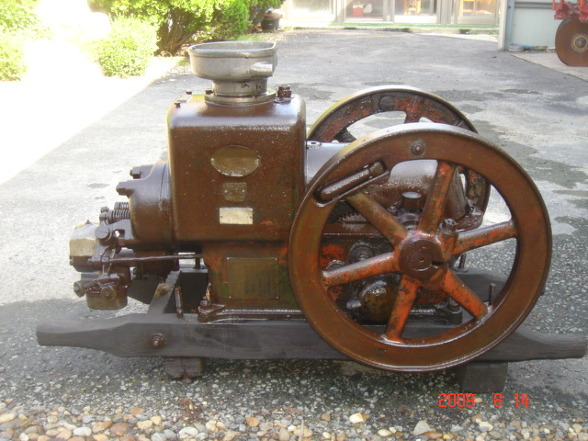
\includegraphics[scale=0.5]{DBs/pic/002.jpg}\\
\caption{발동기는 가장 원시적인 동력발생장치로 무게는 상당하고 발생동력은 작아 현재의 동력발생장치에 비하면 상당히 비효율적이다(양수, 탈곡, 정미기, 방앗간에서 동력원으로 주로 사용).}
\end{figure}


\chapter{나의 어린시절}

1959년 가을 강원도 철원군 신서면 대광리 294번지 방앗간집(현 경기도 연천군 신서면 도신리)\footnote{1963년 행정구역 개편으로 강원도에서 경기도로 편입되었음.}에 새까만 조그마한 천사(10월 4일생)가 태어났습니다. 위로 형이 3명으로 625동이인 장남, 전쟁 후 서울 신촌에서 태어난 2남, 그리고 방앗간에서 3남과 저 이렇게 남자위주의 집안이었습니다.

아버님의 고향은 경기도 장단군 대강면 우근리에서 외갓집이 있는 대광리에 오셔서 정착하시며 가정을 이루시게 되셨습니다.  일제 강점기에 전기공사를 하시고 625당시 기갑부대 상사로 군복무를 하신 경험이 있어 처음에는 큰집에서 운영하시는 방앗간에서 일을 하시다가 정미기의 벨트에 옷이 감기는 사고를 당하셔서 제가 태어난 해에 방앗간 일은 그만두시고 현재의 집으로 이주하시어 온갖 일들을 겪어오셨습니다.

간식거리가 없던 시절이라 옥수수와 쌀 등 곡식을 강냉이기계에 넣어 튀기면 아주 훌륭한 간식거리가 되어 기계 2대를 가지고 밤늦도록 일을 하셨다고 하시고, 또한 형님 두 분은 리어카에 강냉이기계를 싣고 한겨울의 혹한을 견디며 내산리고개를 넘어 마을마다 다니며 남의 집에서 자면서 강냉이를 튀긴 얘기가 지금은 집안 식구들이 모이면 무용담이 되곤 합니다.

간식거리가 늘어나면서 강냉이사업은 주 소득원으로서 한계가 있었지만 저희 어머님은 미련을 버리지 못해 제가 태어난 해부터 30살이 되던 때까지 간간히 오시는 손님을 모아서 강냉이를 튀기곤 하셨습니다.

저도 초등학교를 졸업하고 중학교 입학 전까지 제가 강냉이를 튀기는 일을 하기도 하였습니다.

또한 아버님은 기름도 짜고 국수를 누르는 일도 병행 하셨는데 지금은 공산품으로 다 되어있는 완제품을 사다가 일만 하면 되지만 그때당시에는 철로레일로 만든 틀에 유압잭을 이용하여 볶은깨를 압착하여 기름을 짜도록 직접 제작 사용하시여 기름한번 짜려면 엄청 힘든 유압잭 펌프 작업과 깨를 넣은 주머니가 터져나가지 않도록 예민한 작업을 수반하여야 하는 과정을 거쳐야 하였습니다.

저는 중학교 2학년 때 집에 남아도는 깻묵을 곱게 빻아 종이봉투에 담아 어항의 밑밥으로 만들어 유리어항과 함께 파는 요즘 말하는 아르바이트도 하였습니다.(여담이지만, 그때 모인 돈을 아버지가 좀 빌려달라고 하시고는 아직까지도 갚지는 않고 돌아가셨습니다. 물론 더 큰 것을 많이 받았지만)

그리고 큰형이 1972년 자전거포를 개업하여 자연히 일을 돕다보면 몸에 배이게 되어 그때부터 나의 장래는 기계와 관련한 장래를 생각하게 되었습니다.

중학교 친구들과 같이 놀러 다니는 것 보다는 집에서 항상 농사일과 자전거수리 같은 많은 일을 하였습니다.

모든 사람들이 마찬가지이겠지만 토목, 건축, 목수, 미장 등 지금은 각 분야의 전문가가 와서 보수를 받고 하지만 그때당시에는 전문가가 따로 없는 모든 것을 스스로 해결해야만 하였습니다.

어느 정도규모의 집짓기나 보수정도는 직접 다 시행하였고, 농사일 중에 제일 힘들다고 하는 양잠(누에치기)시설인 잠실 신축과, 식구가 늘어남에 따라 필요한 방들은 아버지와 직접 시공하여 고등학교 진학 할 때는 상당히 일이 몸에 배어 있었습니다.


\begin{figure}[b]
\centering 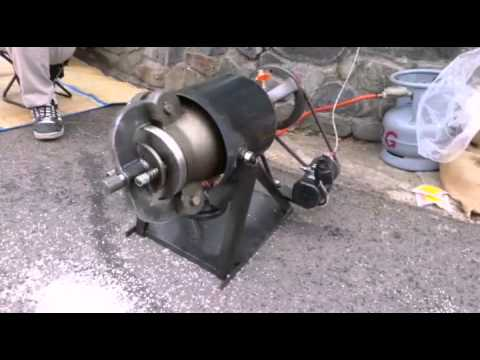
\includegraphics[scale=0.6, trim={1cm 1.8cm 1cm 1.7cm},clip]{DBs/pic/003.jpg}
\caption{\small어린시절 대표간식거리인 강냉이를 튀기는 기계(뻥소리와 동시에 동네 아이들이 뛰어와서 흩어진 강냉이를 주워서 먹는 즐거움이 있었다.}
\end{figure}



\chapter{고등학교 시절}

나의 어린시절에서 조금 언급한 바와 같이 저는 자라온 환경에 따라 의정부공고 기계과에 진학을 원하였으나 가정형편상 어려움이 있어 연천실고 농과에 진학하여 졸업 후 농촌지도소(현 농업기술센터)에 취업을 권유하시여 연천실고 농과에 입학시험을 치렀고, 입학금을 납부하러 학교에 오신 아버지가 입학금을 납부하고 나오셔서 `너 몇 등이나 한 것 같으냐?' 하고 물어 보셔서 아마 상위권에는 있겠죠. 했더니 아버지가 하시는 말씀이 `니가 일등이더라' 하시면서 `너 뭐 가지고 싶은 것 있냐?' 하시기에 탁구라켓하고 네트가 필요하다고 말씀드렸더니 전곡에 가서 탁구장비를 사주셨습니다.

참고로 그때당시에는 『공업입국』이라는 국가의 목표가 있어 각 중학교에서는 성적 상위권의 학생들은 ``금오공고'', ``철도공고'', ``의정부공고'' 등 공업학교로의 진로는 곧 졸업 후 진로가 탄탄하였다고 하여도 좋을 것입니다.

아버지와의 입학금납부 후 많은 생각을 들게 한 것은 나도 능력은 충분한데 내가 진학하고 싶은 학교에 진학은 못하고 진로가 다른 학교에 진학한 것이 불만이 되어 아주 꼴통들만 한다는 밴드부에 자진하여 가입한 것이 나의 인생에 많은 변환점이 되었던 것입니다.

밴드부 연습은 아침조회 전과 방과 후에도 하여 아침연습하고 나면 배가고프니 점심으로 싸온 도시락을 수업 전에 먹고, 점심시간을 그냥 패스, 방과 후 연습을 마치고 집에 가면 배가 너무 고파서 소나기밥을 먹는 일상을 계속하다보니 1학년 말쯤 배가 좀 고플 즈음이면 뱃속이 싸르르 하여 친구아버지가 운영하시는 약방에 가서 말씀드리니 ``위장장애인데 그 나이에 벌써 그러면 어쩌냐!''하시며 걱정하시였습니다.

이때 얻은 위장병으로 평생을 고생을 하다가 이제는 완치되어 건강한 몸으로 복귀되었습니다.

밴드부를 하면서 매도 많이 맞았는데, 선배들한테 매 맞는 것은 그러려니 하다가 담임선생님이 조회에 늦었다고 마대자루를 가지고 풀스윙으로 맞은 것이 불만이 되어 조회 끝나자 친구와 둘이서 기차타고 서울로 도주하여 시청을 구경[지하철 개통(1974년)된 지 1년]하고 집에 돌아왔더니 선생님하고 친구들이 집에 왔다갔다고 하였습니다.

그 이후로 학교생활에 점점 흥미를 잃어 부모님한테 학교 안 다니고 학교 보낸 심 치고 자동차정비학원에 보내달라고 하였습니다. 그 시절이나 현재에도 모든 부모님의 소망은 본인의 자식은 정상적으로 학교를 보내서 졸업하는 것이 바람인데 제가 고집을 꺽지를 않자 1학년 마치고 중퇴를 하기로 부모님께 말씀 드렸습니다.

학교를 중퇴하는 것으로 마무리 짓고 집에서 오토바이 수리와 농사일을 하며 2년여를 지난 후 서울역 옆에 있는 ``한국자동차정비학원''에 6개월 과정의 `자동차정비기능사 2급' 과정을 수료하고 자격증을 취득하고 목동에서 청량리에 다니는 중부운수 버스회사에서 버스정비(월급 5만원에서 식대 2만5천원 빼고 작업복 사고 나면 여유 돈 없슴)를 하는데 버스정비는 운행 특성상 야간정비가 일상인데 가뜩이나 위장병이 있는데다 야간에 야식으로 지급되는 라면을 먹고 나면 심한 속쓰림을 느끼며 버스정비 기술을 배웠습니다.

군 입대 전까지 영등포 문래동에 있는 정비단지 1급공장 엔진부에서 기술을 배우다가 79년도 신체검사결과 ``1급 갑종 현역입영대상''으로 판정되어 수료한 학원에 가서 `기술지원병 입대지원'을 하니 79년 9월 14일 입영영장을 받아 입대하기 위하여 동네 어르신들한테 인사드리고 논산훈련소 수용연대에 갔더니 `병적기록부'가 오지 않아 입대가 불가하다고 하여 다시 서울로 올라와 학원 → 육군본부 → 병무청을 쫓아다닌 끝에 5일 후인 79년 9월 19일 입대를 하였습니다.

\chapter{군복무 시절}

훈련강도가 가장 세다는 논산훈련소 30연대, 나의 고질적인 위장병은 여기서도 나를 힘들게 하였습니다. 불필요한 식욕은 훈련에 지치고 허기진 배를 채우기 위하여 식판에 가득하도록 밥을 퍼서는 그것을 다 먹고 다음날 그게 얹혀서 배가 아파 조교에게 말했더니 `그냥 가볼래 아니면 유급할래' 하기에 `그냥 가겠다.'고 하고 단독군장(철모에 탄띠, 그리고 소총)은 동기 중에 한명이 다 가지고 뛰고 나는 맨몸으로 구보를 하다 보니 체한 것은 해소가 되어 훈련을 마치었는데 그 이후부터는 식사 후 속이쓰린 증상이 계속되어 마침내는 군 생활 중에 위장수술을 하여야 하는 지경에 까지 이르게 되었습니다.

훈련 중에 온 나라를 뒤흔든 사건인 10.26 사건이 발생하였습니다. 훈련병인데도 훈련 중 비상대비로 훈련화도 제대로 벋지 못하는 긴장된 생활 속에 훈련을 받았습니다.

그래도 훈련은 무사히 마치고 각 부대로 배치되는 배출대대에서 복무부대로 배속을 받는데 모든 장병이 ``간다간다 열차00소대'' 하고 선창을 하면 조교가 교번 000번 000, 0000부대하고 호명을 하면 뛰어나가 그 줄에 앉는 것으로 군생활의 운명이 결정되는 것입니다.

그리하여 나의 순간 ``간다간다 열차4소대'' 000번(지금은 교번을 잃어버렸음) 이병 허호강 `육군본부' 하고 배치를 받아 후송열차 타고 용산으로 와서 자대에서 인솔 나온 버스로 육군본부 본부사령실(사단규모)로 그리고 다시 수송대대로 올 때 까지는 그저 소풍 나들이 온 정도로 생각하였는데, 운명의 여신은 주특기인 정비병을 정비중대로 보내지 않고 일반차량중대(대형차량) 버스소대로 배치가 되면서 군생활의 희비가 갈리게 되었습니다.

그때까지만 해도 자동차정비가 나의 희망 진로로서 정비중대로 배치가 되면 정비기술 및 1급 자격증 취득의 기회도 주어지는데 얄궂은 나의 운명은 버스소대에 가서 버스정비병으로서 가장 힘든 군 생활을 영위하게 되었습니다.

이제는 40년 전의 군복무 생활에 대한 이야기로서 부대도 없어지고 보안에 대한 문제가 없을 것으로 생각이 되어 이제는 아련한 추억에 대하여 기술하려고 합니다.

버스소대의 임무는 육군본부 및 예하부대에 근무하는 군인 및 군속들의 출퇴근 및 행사(전투)지원이 주 임무로서 아침 5시기상 바로 식사를 마치고 통근버스로 각자의 노선대로 운행을 하고 8시 전까지 육군본부 본청으로 출근을 시키고, 지정버스 안에서 아침점호 후 일일점검, 주간점검, 월간점검과 아침점호 시 정비요청차량에 대하여 임무를 부여받은 대로 자체정비와 차량세차를 실시하고, 4시부터 다시 본청에서 퇴근운행을 마치고 막사로 이동하여 내무생활로 이어지는 참으로 어려운 군대생활을 하였습니다.

남들이 보기에는 육군본부에서 무슨 군대생활이 어려웠었냐고 하겠지만 소대원 60명 중 70퍼센트는 버스의 운행사고를 줄이기 위하여 하사관이상 장기복무자가 운전하는 차량이 있고, 사병 14명이 일부노선 운행과 부사관의 결행이 있을 시 대체하고, 정비와 세차를 담당하는 것이 주된 임무로서 지금은 대형차량도 모든 작업은 첨단장비를 사용하지만 하루에 3대 이상의 차량 클러치 작업을 하다보면 100㎏이 넘는 트렌스밋션을 맨손으로 들었다 놨다 하고, 펑크수리도 수차례의 곡괭이질과 휠너트를 풀고 조이기 위한 휠복스는 어깨의 힘과 공구무게의 반동을 이용하는 작업은 공구의 무게만도 한 20㎏씩이나 되어, 대형차량 정비는 공구를 들고 다니는 것만으로도 힘겨운 작업이었습니다.

거기에 위장병이 있는 나로서는 추위 속에 바람이 세차게 몰아치는 차 밑에서 작업하는 것이 큰 고통으로 느껴지는 게 일상생활이 되어버려, 이등병때는 군기가 바짝 들어 위장병 따위는 육군본부 의무대에서 약 타다가 먹는 정도로 지내야 했습니다. 12.12사건 전에 육군본부 의무대로 약을 타러 갔는데 군의관들이 후다닥 뛰어 내려와 뭔 일인가 했더니 참모총장인 정승화 장군이 의무대를 방문한 것이었습니다.

이등병이 장군을, 그것도 참모총장이 앞으로 지나가다 내게로 와서 `집이 어디냐, 어디 아파서 왔냐' 하고 물어 보아, ``경기도 연천에서 왔습니다. 배가 아파서 왔습니다.''하고 복창을 하니 어깨를 툭툭 치며 빨리 낳으라고 격려하시고 가셨는데, 그 며칠 후 12.12라고 하는 엄청난 사건이 그 현장에서 벌어져 정승화 장군은 이등병으로 예편되었다가 문민정부에서 사면복권되는 사건이 있었습니다.

12월 12일, 그날 제가 근무하던 육군본부 본부사령실장병은 육본강당에서 있었던 군악대와 여군단본부에서 개최하는 음악회를 보고 있었습니다. 중간 쯤 진행(저녁 8시경으로 기억됨) 중에 중령인 듯 보이는 장교가 무대로 올라와 `전 장병은 지금 즉시 자대로 복귀하라'고 하여 복귀하니 그때부터 출입금지, 그리고 야간 동초근무를 내려간 선임병은 교대를 하지 못해 온밤을 혼자 근무하였습니다.

10.26의 여파로 육군본부 본부사령실 내에는 20사단에서 파견 나온 부대가 데모진압을 위하여 훈련을 하며 상주하였는데, 12.12사태로 이번에는 육군본부와 국방부를 무장해제 시키고 공수부대원이 상주하게 되었습니다. 10.26사태 이후로 모든 군인은 계엄군이라 하여 특식으로 계란 1알, 사과 1알, 보름달 카스테라 1봉지를 매일 특식으로 지급받기도 했습니다.

이어서 지금껏 논란이 계속 이어지는 5.18사태도 발생하여 그 당시 병력수송을 지원했던 부사관들의 얘기로는 광주를 다녀온 군인들이 눈빛부터 다르더라는 것이 화제가 되곤 하였습니다. 

아무튼 그 어렵다던 군생활도 나름대로 나의 행운인지 능력인지는 모르겠지만, 이등병으로 자대배치 받고 채  일백일도 되기 전에 모범사병 특박이라는 혜택을 받아서 집에 가보니 저의 입영일에 탄생한 조카가 백일이 된다고 하더라고요.

이어서 군대생활에 대한 나의 특별함은 시력이 좋아서인지 본부사령실 전투력측정에서 일반차량중대(트럭소대, 버스소대) 사격선수로 출전하여 카빈소총은 기지거리 6발 사격에서 100\%, 일병때 지급받은 M16소총은 20발에서 95\%정도 명중률을 가져 포상휴가 3박4일(군 생활은 뻥이 많다고 하니 믿거나 말거나) 받고, 또한 그때는 유류파동 및 고춧가루 파동으로 반공 및 에너지절약에 관한 수송대대 웅변대회가 있었는데 우리 중대 병력은 학력이 거의 중졸정도인지라(저도 중졸이지만) 일반차량중대 대표로 출전하라고 하여 웅변대회에도 출전하여 2등 입상이라는 영예와 함께 또 포상휴가를 받기도 하였습니다. 

또한 타고난 저질체력이라 뜀뛰기는 항상 뒤에서 1등만 하던 것도 군복무생활을 하면서 단체구보에서 한 번도 낙오되지 않는 체력을 갖게도 되었습니다.

그러던 것이 다시 80년도 가을이 되면서 위장병으로 고생을 하는 것을 고참병들이 보고 내무반에 올라가서 좀 쉬라고 하여 내무반에 들어가니, 내무사열 준비로 고참병들이 청소를 하고 있어 같이 하려고 하니까 침구를 깔아주면서 ``넌 좀 쉬어'' 하는 소리에 눈물이 왈칵 쏟아지면서 그만 소리 내어 울고 말았습니다. 평상시에 고참병들은 후임병을 괴롭힘의 대상으로만 하고 우리 버스소대의 경우에는 안전을 우려하여 군기가 상당히 엄하기로 알려져, 버스소대 만큼은 유격훈련도 열외되기도 하였습니다.

그 이후로 국군서울통합병원에 지원 나가는 버스를 타고 내과 외진을 받으니 당시에는 보통 위장검사는 ``위 투시(조형제를 마시고 X선 촬영으로 진단)''가 최선이었는데 검사 후 약을 처방받아 복용을 하는데도 낫지가 않자, 그때부터 보급되기 시작한 위내시경(호수가 엄지손가락보다 더 굵었던 것으로 기억남)으로 검사를 하니 십이지장궤양인데 수술을 하는 것이 좋겠다고 하여 아버지한테 전화를 드려 `면회 좀 오셔 달라'고 하여 수술여부에 대하여 말씀드리니 `요즘 의술이 좋아서 수술을 하는 것이 좋겠다.'고 하셔서 수도통합병원으로 후송 가서 수술을 하고 부산통합병원으로 이송 입대, 18개월 만에 의병제대를 하게 되었습니다.

저희 아버지도 70년대 초반에 술도 안 드시는데 먹은 음식이 체하고 그 후유증으로 위를 80\%를 절제하는 수술을 하신 경험이 있어 현대의술에 대한 믿음이 있으셨던 것 같습니다.

지금 돌이켜 보면 현재의 의약품이면 간단하게 치료되는 위장병이 그 당시에는 그렇게 수술을 하여야 하는 것인가 하고 의구심이 들 때가 많이 있습니다.

81년 2월에는 대통령선거인단에 의한 대통령 간접선거가 있어 휠체어를 타고 투표소에 가서 대통령선거인단 투표를 한 기억이 지금도 또렷하게 남아 있습니다.

\chapter{방황의 시절}

1981년 3월 전역을 하고 아버지를 도와 농사일을 하다가 8월에 연서농업협동조합(연천농협과 신서농협 통합으로 현재의 연천농협) 농기구수리센터가 신설되는데, 제가 소지한 자격증의 대상자를 직원으로 뽑는다고 하여 농협에 입사, 수원에 있는 농촌진흥청 교육원에서 2주 농기계수리에 대한 교육을 수료하고 연천경찰서 맞은편 연서농협 농기구수리센터를 개설하고 근무를 하는데, 그 당시에는 농기계라고 해야 기껏 경운기나 이앙기 정도의 초보적인 정도라 활성화도 되지 않고 하여 회의를 느끼고 있다가, 아버지한테 자동차 정비기능사 1급 자격증을 따고 창원에 있는 기능대학(현재는 `폴리텍대학' 이라고 함)에 가고 싶다고 학원에 보내달라고 해서 농협입사 6개월 만에 퇴사 서울에서 공무원생활과 학업을 병행하고 있는 3째형 자취방에서 같이 생활하면서 군입대 전에 다니던 학원 1급반에 등록 학원을 수료하고, 2번인가의 시험에 낙방을 하니 뒷받침이 힘드신 아버지가 내려와서 같이 농사 짓자고 하여 더 이상 배우고자 한 것은 접고 아버지와 같이 농사를 시작하였습니다.

그때 당시의 농사규모는 대광골 밭 1,500평(4,500㎡)에 심은 뽕나무로 누에를 봄·가을로 치는 양잠과 답곡리에 논 3,000평(9,000㎡), 밭 5,000평(15,000㎡)로 아버지가 어머니와 두분이 경작하기에는 상당히 힘든 정도이고 제가 아버지와 같이 농사를 시작하니 제 목으로 암송아지 2마리를 구입 본격적으로 농업에 종사하게 되었습니다.

4계절 구분 없이 아버지와 함께 낮에는 농사일을 밤에는 큰형이 운영하는 오토바이센터에서 일을 하던 중 군대에서 수술한 후유증인지 가을누에 4령(4잠잔다고도 함)기  왕성한 먹이활동시기에 오전에 뽕따러 갔다가 ``배가 아파서 저 먼저 집에 갈게요.'' 하고 먼저 내려와 볼일을 보고 점심 뽕잎을 주는데, 계속 아파지고 점심밥을 먹는데 도저히 먹히지는 않고 해서 큰형과 동두천 서울병원에 외진을 갔더니, 수도통합병원에서 군의관으로 복무하면서 내가 수술 받을 때 같이 참여하였던 대위가 전역 후 내과 과장으로 진료를 보는데, 나를 알아보고는 급성위염이라고 진단하여 처방약을 가지고 집에 왔는데 도저히 물도 넘어가지 않아 토요일 큰형이 가지고 있던 브리샤픽업을 타고 의정부 성모병원으로 진료를 하러가니 충수(맹장)염으로 바로 수술하여야 한다고 입원하였는데 토요일과 일요일은 수술을 못하고 월요일에 수술을 하니 맹장이 터져 복막염으로 되었습니다.

의사가 환자를 보는 관점이 자기가 수술하였던 환자라고 해서 속단한 오류가 초기에 원인치료를 하면 간단한 수술로 끝날 수 있었던 것을 오진으로 몸은 몸대로 고생하고 수술비용도 많이 들고 회복기간이 상당히 늘어나는 결과가 되어버렸습니다.(81년도 농협에서 급여가 168,000원이었는데 수술비가 백오십만원이 나왔고, 15일 입원과 퇴원 후 2달가량 수술부위를 치료하여야 하였음)

아버지와 함께 농업을 계속하던 중 1984년 장마철에 병원에 좀 다녀오신다고 하고 저는 어머니랑 같이 논에 풀 뽑으러 갔는데, 종일 비를 맞으며 논김을 매다보니 오후 3시쯤 하도 추워서 어머니한테 집에 가자고 해서 오는데 집 앞에 사는 형이 아버지가 위독하시다고 연락이 와서 의정부신천병원에 도착하니 주사쇼크로 그날로 운명하시었습니다.

아버지 장례를 치루고 나니 그 충격이었는지 큰형도 허리가 아파서 운영하던 오토바이센터도 못하게 되었고, 저 또한 어머니하고의 의견차이 때문에 농업에 전념할 수가 없었는데 송아지 두 마리가 새끼를 낳고 또 비육우로 젖소 숫송아지를 하나 더 늘려 5마리와 양잠을 위한 뽕나무밭은 수익성이 떨어져 다 캐서 원래의 밭으로 만들어 신망리에 계시는 외갓집 4촌형님의 도움을 받아 무를 심어 일을 하는데, 어머니하고의 의견(성격)차이는 도저히 같이 있을 수가 없어서 농사 짓던 것을 걷어치우고 동두천에 택시운전을 하러 나가버렸습니다. 

택시운전을 하면서 장래를 위해서는 정비를 계속하여야 하는데 당장 눈앞의 소득에 이끌려 택시운전을 하였는데 그때당시의 정비사 월급은 월 1십만원 정도이고 택시기사들이 간간히 주는 팊이 수입의 전부이고, 택시기사는 월 오십만원은 기본적으로 수입이 확보되어 있어 그 유혹을 이겨내기가 힘들었던 것 같았습니다. 

85년도 버스운전기사와 덤프트럭운전기사들은 보통 9십만원에서 1백5십만원 정도의 수입이 있었습니다. 

하지만 택시운전하면서 아무리 수입이 높다 한들 혼자 무계획적인 삶을 살게 되면서 저축도 되지 않고 무절제함에 지쳐가다, 어머니는 3째 형네 집으로 조카를 봐주시러 서울로 가셔서 방황을 마치고 다시 농사를 지으러 대광리로 돌아와 이앙기, 콤바인 등 농기계를 장만하여 친구들과 같이 어울려 농사일에 열중하고 있었는데, 1988년 가을에 의용소방대장으로 있던 친척아저씨가 군청에서 니가 가지고 있는 자격증소지자 채용공고가 났는데 농사짓는 총각으로 결혼하기도 힘든데 공무원시험 한번 봐보라고 하시기에 콤바인은 계속 일을 하여야 하기 때문에 친구와 동네 후배한테 콤바인 일을 맡기고 콤바인 작업하는 동안에 논두렁에 앉아서 국사와 국민윤리책을 보면서 공부하였는데, 국사는 도대체 어찌 공부해야 할지 몰라 하고 있는데 사학과를 다니는 6촌동생이 놀러왔다가 요점을 딱 짚어주니 그게 큰 도움이 되어 무난히 합격하게 되었습니다.

88년도에 콤바인은 일년에 40일 정도 일을 하고, 하루 일을 하면 15만원정도의 수입이 있고, 이앙기도 20일정도 일을 하고, 하루에 10만원의 수입이 있었는데, 쌀값은 80㎏ 1가마니에 18만원이었습니다. 

환산에 도움을 주기 위하여 잠깐 표로 만들어 봤습니다. 

\begin{figure}[h]

{\centering연간 총소득 산출내역(1988년)

\tabulinesep=1.2mm
\begin{tabu}{|X[1,c]|X[1,c]|X[1,c]|X[1,c]|X[1,c]|}
\hline
주수입원 & 콤바인 & 이앙기 & 경운기 & 벼농사 \\ \hline
단가/일 & 150,000 & 100,000 & 50,000 & 40가마/80㎏ \\ \hline
작업일수/연간 & 40 & 20 & 20 & 180,000 \\ \hline
연간소득금액 & 6,000,000 & 2,000,000 & 1,000,000 & 7,200,000 \\ \hline
\end{tabu}}
※ 연간 총소득 대비(농업경영 : 공무원)
\begin{itemize}
   \item 농업소득 : 16,200천원(총 소득금액) - 6,200천원(농자금) = 10,000천원
   \item 공무원 소득 : 본봉 168,000원(8급 2호봉) × 16개월(기말수당 4회포함) = 3,024천원\\%
                  여비, 급식비 등 제 수당 50,000원 × 12개월 = 600천원 \\%
                  본봉 3,024천원 + 제 수당 600천원 = 총소득 3,624천원
   \item 소득대비 : 3,624천원 – 10,000천원 = -6,376천원
\end{itemize}
〈80년대 주요 직업별 월소득 : 버스, 덤프(90만원 \textasciitilde 150만원), 택시(50만원), 보통인부(일당 2\textasciitilde3만원)%

※ 기억에 의한 수치임으로 실제의 경제지표와는 차이가 있음 
\end{figure}

\chapter{어공 시절}

\begin{figure}[h]
\centering 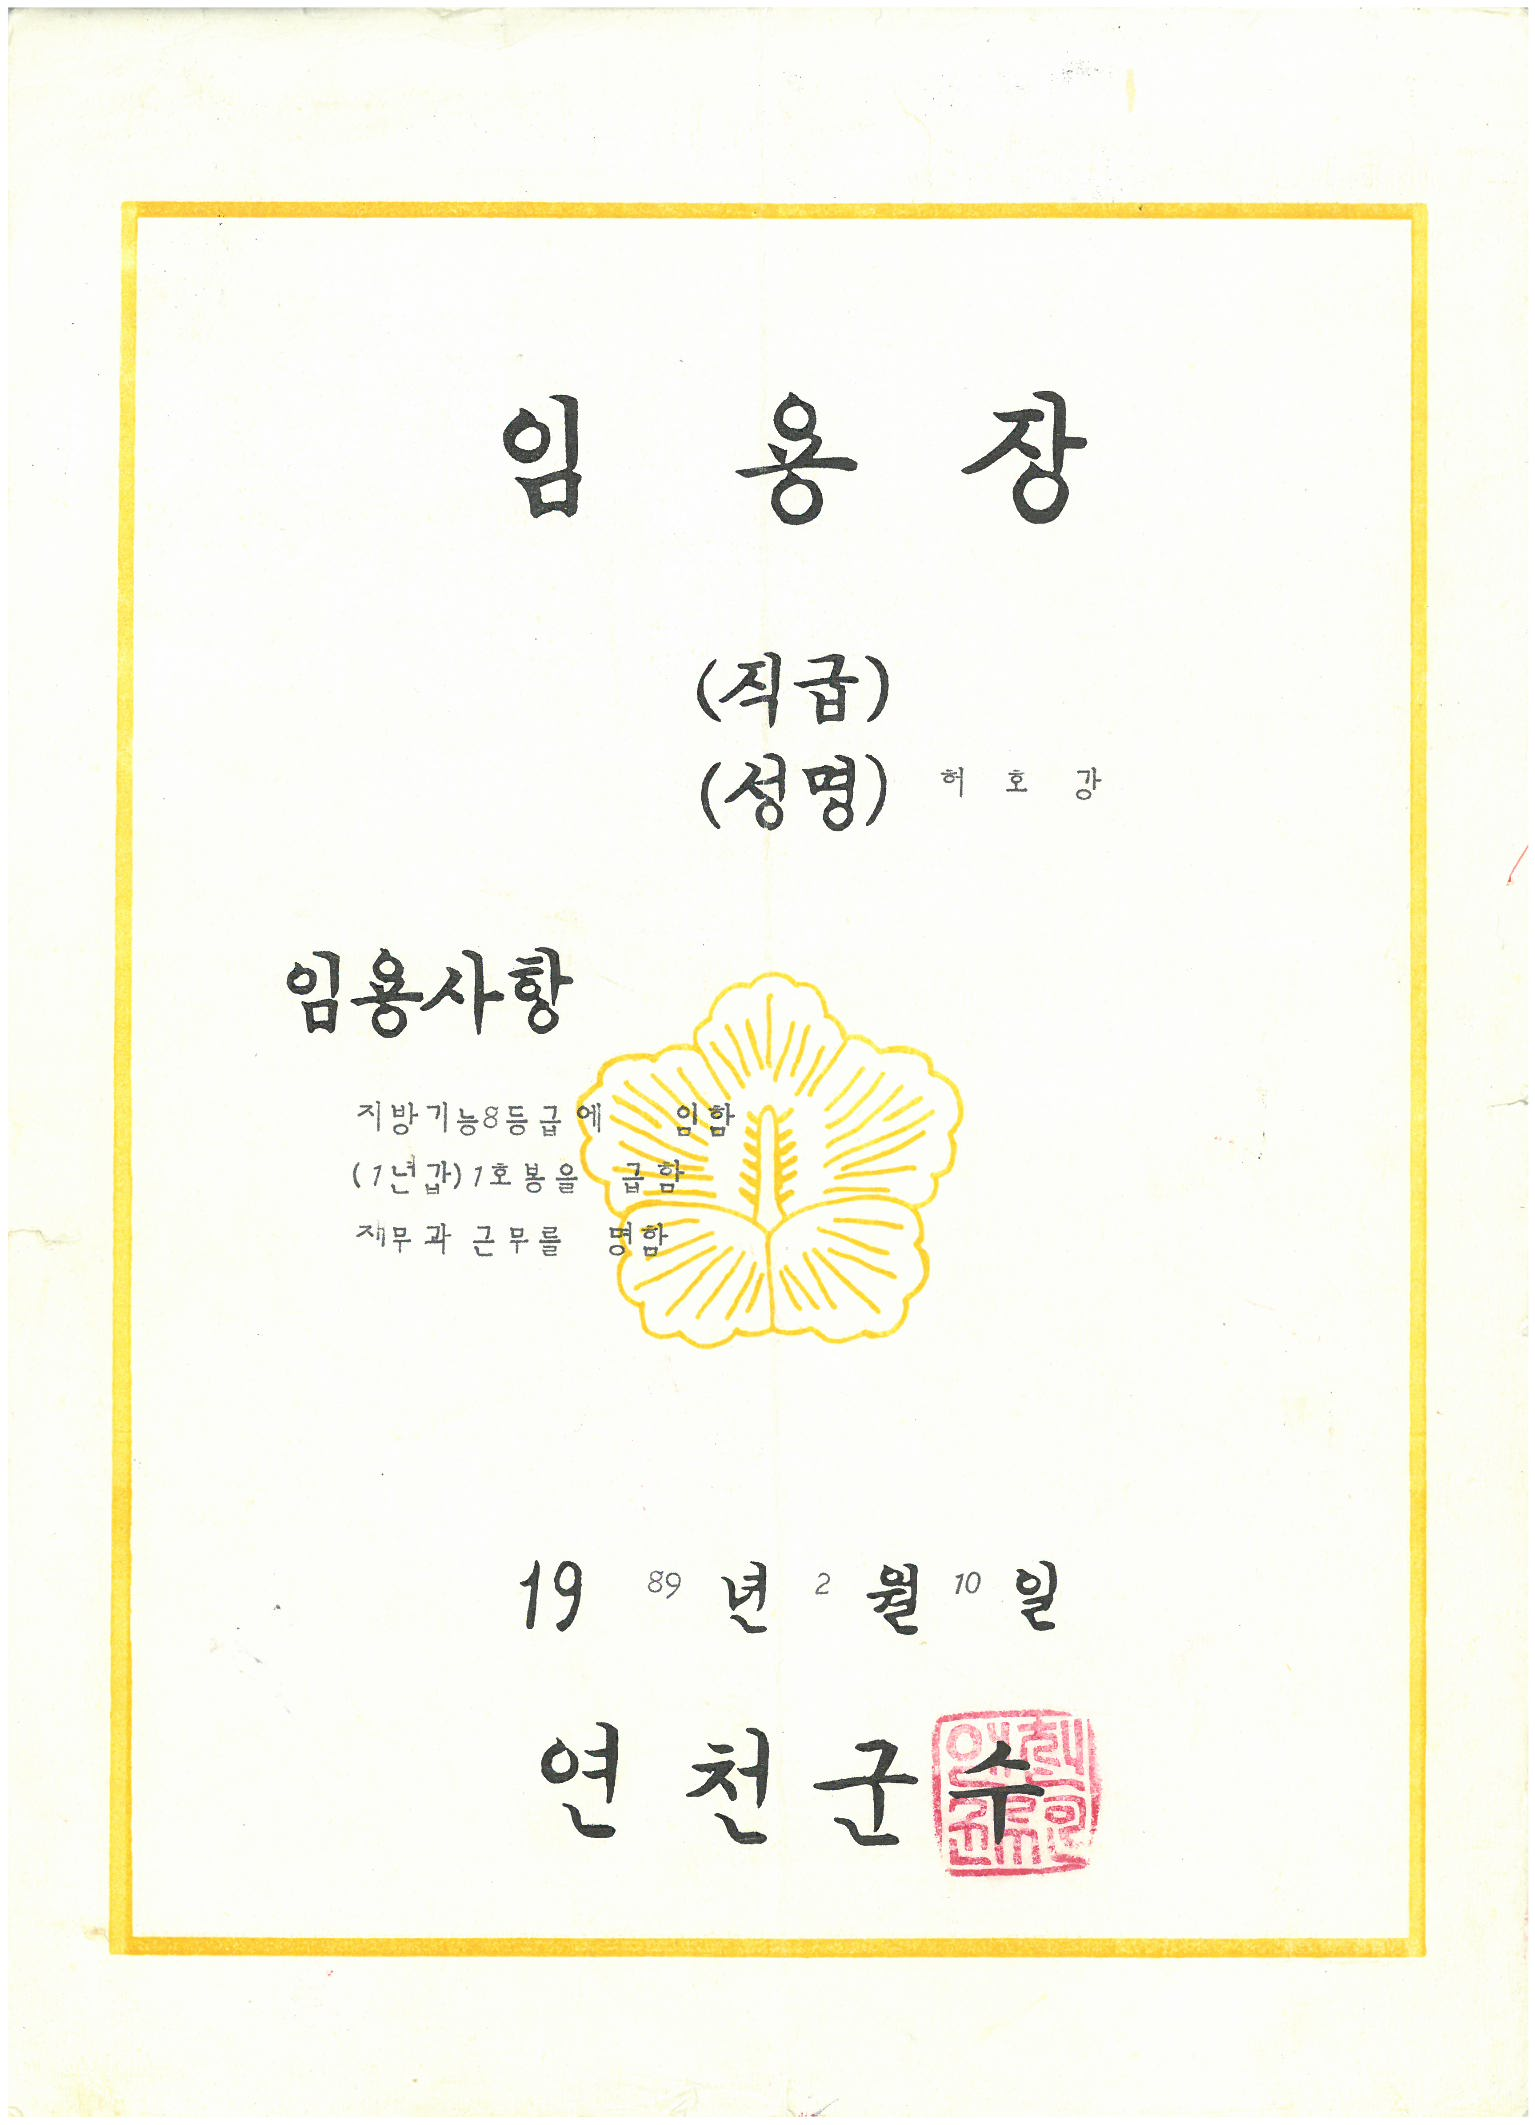
\includegraphics[scale=0.3]{DBs/pic/004.jpg}\\
\end{figure}

1989년 2월 10일, 연천군청 재무과 경리계(지금의 도시주택과 사무실) 담당업무는 관용차량관리! 관리대상은 관용차량 90여대와 재무과 소속 운전원 20여명에게 배차 및 복무관리 초임발령 당시 31세 그래도 사회에서 다양한 경험을 쌓아온 나이 많은 노총각이었었는데 배차대상 운전원의 최연소자가 3년 선배님들 그리고 그 위로 곧 퇴직을 앞두신 분들까지…

그래도 배차나 차량관리에 많은 분들이 협조하여 도와주시고 같이 의논을 거쳐 업무를 수행하다보니 그 당시에는 자가용을 소유한 직원들은 아예 없던 시절이라 업무를 수행하면서 관용차량 배차가 절실한 시절이라 주어진 업무에 비하여 상당한 비중을 가지고 있었던 것 같았습니다.

임용 후 첫 급여일인 20일 채 10만원이 되지 않는 보수명세서를 보고 이런 직장을 계속 다녀야 하나 하는 생각을 하며 하루 이틀 사흘… 이렇게 지나다 보니 나름대로 직원들과 어울리며 생활도 하게 되고…

또 지금도 기억나는 것은 현재의 우리는 사무용품 홍수 속에서 근무를 하고 있지만 기안용지(갑),(을)로부터 시작해서 출장신청서 지출결의서 등 모든 공문서식과 함께 칼, 콤파스, 지우개, 수정액, 타자기리본, 복사용지 등  각 실과소에서 필요로 하는 사무용품 전체를 1년에 한번 경리계에서 일괄신청을 받아 조달요청을 하면 조달청에서 대형화물차로 군청 마당에 하차해 놓고 각 실과소 주무계 서무담당에게 수령하라고 하면, 전 직원이 나와서 물품을 수령해 가는 데 배분하다 보면 주문한 수량하고 배부한 수량이 맞지 않는 것이 당연한 듯 집어가고, 나이 어린 직원들은 남녀불문하고 ``허주사님 자 하나 주시면 안 돼요?'', ``칼 하나 주시면 안돼요?'', 하면서 아양 떨기도 하고… 물품 숫자가 영 안 맞으니까 ``신분들은 공무원인데 하는 행동은 강도들이네'' 하고 웃으며 농담도 하였던 기억이 아련하네요.

`어공'에서 `늘공'으로 전환되는 계기가 된 민원실의 민원담당 여직원이 행정전화번호부에 이름이 희한한 직원이 있었는데, 내 이름도 평범하지는 않고 그때는 `지역의료보험조합'과 `공무원교직원 의료보험조합'이 별개로 운영되던 때라 지역의료보험 해지를 위하여 `재직증명서'를 발급받아 의료보험조합에 제출하여야 하기에 민원실(지금의 군청마당 가운데 공원 위치)에 가서 재직증명서를 발급받아 사무실 책상에 두었다가 두서너 시간 지난 후 의료보험조합에 제출하려고 찾아보니 없어서 다시 민원실에 가서 재직증명서를 발급신청 하니 아마도 ``뭔 이런 정신나간 사람이 있나'' 하고 생각했을 것입니다.

1989년 4월 1일(토) 연천군 백학면 ``원당출장소''가 ``장남면사무소''로 승격되어 군수님 축하화분을 전달하러 장남면사무소에 경리계 차석(윤종훈 전실장님)과 함께 전달하고, 귀청하는 도중에 민원실 여직원이 살던 미산면 우정리 ``왕산상회''에 들러서 라면이라도 먹고 가자고 하여 들렀는데 마침 혼자 집에서 가게를 보고 있어 라면 끓여먹고, 막걸리 마시고....(당시의 경리계 주 업무는 의전용 물품 조달이 계약지출보다 더 중요하였음)

그리고 정작 역사의 시작은 ``1989년 4월 5일 식목일'' 연천읍 와초리 식목행사장 그때는 식목일이 국정공휴일이라 전 직원이 식목행사에 참석하여 나무심기를 마치고 두부에 막걸리를 마시고 있는데 `산불이 근처에서 발생' 참석자 전원이 산불진화 출동하였는데 저는 그때 출동을 못하고 있다가 민원실 여직원이 운전을 할 줄 안다고 하기에 `그래 운전을 할 줄 안다고 그럼 전부 귀청한 뒤에 한 번 해봐' 하고 군청에 귀청하고 차량의 부속을 사러 전곡에 갈 일이 있어 포니픽업이라는 재무과 차량의 운전석에 앉아서 운전을 하라고 시켰습니다.

\begin{figure}[t]
\centering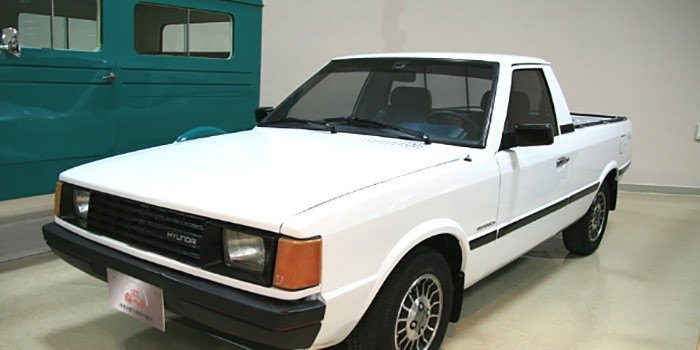
\includegraphics[scale=0.4]{DBs/pic/005.jpg}\\
\caption{어공을 늘공으로 바꾼 문제의 포니픽업}
\end{figure}



지금은 누구라도 면허증은 필수이지만 그 시절에는 자가용은 물론 일반인이 면허증의 간절함이 없던 시절이라 직원들도 별로 면허증을 취득하지 않았고, 또한 나이도 어린 여직원이 운전을 할 줄 안다고 하니 호기심에 해 보라고 한 것인데, 아무튼 정문을 통과하는데 그 옆에 있던 당직자 및 직원들이 손을 흔들어 주었는데 그것이 잘 해보라는 축복의 인사인지 아니면 놀리느라고 손을 흔들어 주었는지 분명치는 않지만 그것이 계기가 되어 서로 관심을 가지고 만남을 계속하고 있었는데, 대광리의 내 방에 있는 전화기로 전화가 와서 받아보니 민원실 여직원,

\begin{quote}
``뭐하시고 있어요.''

``대문고치고 있었는데.''

``집에 대문이 있어요.''

``시골인데 대문이 있지!''
\end{quote}
나중에 확인된 사실은 태어나서 왕산상회에서만 살다보니 대문이 필요 없는 집이고, 우리 집은 농가집이라 마당이 있고 대문이 있는데, 우리 오토바이센터에서 드럼통을 잘라 펴서 만든 대문이라 수시로 용접도 해야 하고, 페인트도 칠해야 하는 그런 그렇고 그런 낡은 집이었지요.

그렇게그렇게 만남을 이어가고 있을 때 그 여직원의 아버지는 전곡우체국에 국장으로 근무하고 계셨는데 마침 사무관 시험을 앞두고 있었는데 이 막내딸이 귀가시간도 늦고 그러는 것이 신경이 쓰이셨는지 양지다방(군청 앞 우박막국수 가기 전 위치)에 오셔서 ``나 오양 아버지인데 이리로 좀 나와요''하셔서 나갔더니 우리 딸하고 만나고 있나 본데 공무원으로서 행동을 주의해서 하라고 하셔서, ``예 주의하겠습니다.'' 하고 그날은 그리 끝났는데,

점점 만남이 잦아지고, 귀가시간도 점점 불규칙한 것이 아버님의 심정을 자극하여 다시 한 번 양지다방으로 오셔서 저를 불러서 ``자네 먼저도 말했는데 왜 행동에 주의를 안하나.'' 하셔서, 그동안에 들었던 이야기도 있고 해서 ``아버님께서 저희 결혼을 안 좋아 하신다고 들었습니다.'' 고 말씀드렸더니, 그 자리에서 바로 수첩을 꺼내시더니 1989년 6월 10일(토) 이날을 가르치시며 ``이날로 결혼 허락받아와'' 하셔서 저희 어머니하고 큰형한테 말씀 드렸더니 이게 웬 횡재냐 하고 바로 허락하셔서 며칠 후 양가인사를 하고 약혼식도 생략하고 바로 결혼식을 하게 되었습니다.

 재무과장님(인사팀장의 장인어른)께서 관선군수님 이시던 군수님에게 주례를 부탁드렸더니 군수님이 제 이력을 보시고는 ``이 사람은 장가가려고 군청에 들어왔나.'' 하시면서 주례를 맡아 주셨습니다. 

그도 그럴 만한 것이, 나이는 31 : 22, 학력은 연천중졸 : 의여고졸, 공무원 경력이 \mbox{4달 : 2년}, 이러한 격차를 가진 남녀의 주례를 선다는 것이 궁금하셨나 봅니다.  발령일로부터 4달, 알기시작하기 시작하여 2달 이렇게 초스피드의 결혼으로 인해 다시는 공무원생활을 떠날 수 없게 된 것입니다.

저희 결혼 이야기는 이 후에도 근 20년간 식목일이면 회자되고 하였던 것이 이제는 역사 속의 이야기가 되었고, 주례를 맡아주셨던 군수님이 내무부 연수원으로 전근 가셔서 직원들을 대동하고 청산면 초성리 열두개울로 워크숖을 오셨는데 제가 그 때 도와주기 위하여 서빙하고 있는데 전임 군수님이 저를 부르시더니 직원들에게 제 소개를 하며 주례까지 서시게 된 이야기를 들려 주셨습니다.

\chapter{늘공 시절}
\section{1990년대}

그렇게 저의 직업인으로서의 공무원생활은 시작되었습니다.

경기도 연천군 신서면 도신리 294-16, 연탄 아궁이에 방 하나 부엌 하나 마루가 있는 단칸방 집에 장롱 하나에 화장대 하나, 그리고 넷이 앉아서 상하나 놓고 밥을 먹으려면 등이 벽에 다 닿는 그러한 스레트블럭 집에서 시작한 신혼살림은, 그래도 저의 둘째형의 집이여서 거주에 소요되는 비용이 없어 부족한 것이 없이 적은금액이라도 저축을 하며 지냈습니다.

1년 후, 모든 가족의 축복 속에서 첫째를 분만하러 의정부성모병원(지금의 의정부역 서부광장 맞은편에 있었음)에 입원하였는데, 자연분만은 어렵고 수술로 분만하여야 한다고 해서 보호자 동의를 하고 수술을 하였는데, 상당한 장애를 가진 아이가 태어나자마자 잘못되어 우리 가족 모두가 놀라고 저는 하늘이 무너지는 심정으로 있었는데, 그래도 산모를 걱정하는 양가의 가족들이나 직원들도 모두 산모가 힘들어할 것이니 입원기간동안 휴가처리 하고 산모를 잘 돌보아 주라고 하여 일주일 간 산부인과 입원실에서 꼬박 같이 있다가 마음을 다스리고 다시 일상으로 돌아 왔습니다. 그 때의 충격은 내가 살아오는 동안 무엇을 잘 못한 것이 있어 이런 시련이 찾아 왔나 하는 반성의 계기도 되었었습니다.

그렇게 어려움은 극복되어 1년 후 그리고 또 2년 후 나름대로 건강한 아들 둘을 두어 목메달을 달게 되었으며, 지금은 각자의 길을 나름대로 노력하며 열심히들 살고 있습니다.(딸2 + 아들1 = 금메달, =  딸2 = 은메달, 딸1 + 아들1 = 동메달, 아들2 = 목메달)

1990년대에는 크나큰 사건도 많이 일어났었는데, 1995년 여름 신서 지역의 집중호우로 인한 동막골 계곡의 인명피해, 1996년 연천군과 파주군(현재 파주시)의 수해, 3년 후 1999년 다시 수해가 발생하였습니다.

\subsection{동막골 계곡 인명피해}

그 전날 당직근무를 하면서 7시경 각 읍면에 전화로 강우량을 보고받아 일지에 기록을 하는데 각 읍면이 10mm \textasciitilde 20mm 미만으로 보고를 하는데 신서면에서는 180mm를 보고하여 `무슨 180mm야 18mm겠지'라고 생각 하였는데, 8시 되기 전에 소방관이 당직실로 전화를 걸어 헬리콥터를 지원하여 달라고 하는데 마침 내무과 행정계에서 동향업무를 보는 친구가 일찍 출근하여 군부대에 헬리콥터를 요청하여 구조지원이 되었으나, 동막골 계곡의 급격한 물 흐름은 다수의 인명이 휩쓸려 실종되어 그날로부터 수일 간 동막골 계곡의 다리부터 파주시 경계인 비룡대교까지 전 직원이 동원되어 수색작업을 하였습니다. 

\subsection{1996년 수해}

1996년 7월 27일부터 강원도 철원군부터 연천군까지 집중된 호우로  인하여 28일 신서면을 비롯해 연천군 전역과 파주시(특히 문산읍)까지 침수되어 엄청난 피해를 입혔는데, 통현리 농협주유소 옆 3번국도가 유실되어 구도로(통제에서 고포리의 농로)로 대형화물차량으로 지원되는 구호물품들이 한꺼번에 몰려들어 정체가 극심해 전곡으로 물품 하나 구하러 가려고 하면 한나절이나 소비되는 극심한 체증과 또한 군청의 지하층에 있던 식당, 전기실 및 문서고까지 잠겨 모든 기능이 마비, 특히나 같이 근무하던 직원은 어머니 집과 자기가 사는 집 직장인 기계실까지 잠기는 바람에 엄청난 고통을 겪기도 하였습니다.

밤낮없이 쏟아져 들어오는 구호물품에 직원들은 기진맥진 하면서도 전 직원이 혼연일체가 되어 각자 수해복구를 하는데, 연천읍내 식당들도 모두 침수가 되어 식사가 가능한 식당이 없어 직원들도 구호급식소에서 식사를 해결을 해야 했는데, 일부 중앙지 언론에서 자기들도 급식소에서 식사를 하면서 연천군청 공무원이 급식소에서 식사를 한다는 기사를 써서 참으로 난감한 일도 겪어야 했습니다.

\subsection{일반직으로의 전환}

기능직 8등급으로 신규 임용되어 7년5개월 만에 7등급으로 1등급 승진, 일반직이라면 9급으로 입사하여도 5호봉 주사보가 가능한 기간에 1등급만 승진. 참으로 공직에 들어와서 왜 이런 차이가 있나 하던 차에 1996년 8월 수해복구가 한참 진행 중일 때 부군수님(당시 참으로 깐깐하다고 하신 분)이 이번에 일반직 전직시험이 있으니 공부 열심히 해서 전직할 수 있도록 하라고 말씀하시고, 또한 행정계장님(지금은 고인이 되셨음)도 이번 기회를 놓치지 말고 해보라고 하여 과목을 보니 기계일반, 기계재료, 물리과목이 있는데 기계관련 과목은 예전에 배웠던 전력도 있고 하여서 무난한데 물리는 배워보지도 못한 과목을 공부하려니 참으로 눈앞이 깜깜… 지금은 인터넷강의라던가 CD강의 등 쉽게 접할 수 있는 것이 교재 한 권, 참고서 한 권을 사가지고 평소에는 다니지도 않던 도서관이라는 곳에 가서 자리 잡고 앉았는데 자세도 잡히지 않고 $F=ma$로 시작하여 플레밍의 왼손, 오른손 등 골치 아픈 공식이 가득한데 이해도 되지 않는 공식을 가지고 자꾸 보다보니, 머리가 지끈지끈하여 잠시 누워 자다 일어나서 다시보기를 반복하여 겨우 시험을 치러 이듬해인 1997년 1계급 강등 된 기계서기(8급)으로 임용되었습니다.(현재는 강등 없이 수평으로 전직이 됨)
\subsection{99년 수해}
1999년 7월 31일(토) 퇴근하고 전곡주유소 옆 수도공무소에서 볼일 좀 보고 있는데 5\textasciitilde6시경 골목으로 발이 잠길 만큼 비가 쏟아져 흘러가 96년 수해경험이 있어 진상리, 삼거리방면 도로가 침수되었다 하여 연천으로 돌아서 선곡리 맑은물관리사업소로 들어가자, 수해가 발생하기 시작 밤 10시경 정전이 되고 무정전전원장치도 일정시간이 지나 완전히 암흑이 되어 구내식당에서 접시에 식용유를 붓고 실장갑을 풀어서 실을 만들어 식용유에 넣어 호롱불을 만들고, 다행히도 전화는 소통이 되어 수시로 재난상황실에 상황을 보고하였고, 한국전력에서는 침수된 도로를 헤치고 전력을 복구시켜 가장 낮은 곳에 위치한 취수장에서 임진강 수위를 보니 취수장 바닥에 거의 도달되어, 지금은 고인이 된 친구와 취수펌프의 모터 2개를 분리하여 한 대는 건설용 선반위에 올려놓고 한 대는 호이스트라는 전동 견양기(호이스트)에 걸어서 올려놓고 밖으로 나와 보니, 취수장 바닥으로부터 50㎝가량 물이 올라와서 철문셧터로 들어오는 물을 막기 위하여 비닐과 모래주머니로 셔터와 철문을 막고 전선관을 타고 들어오는 물은 배수펌프로 강제배수하고 날이 밝아오니 수위도 낮아지고 직원들이 출근하여 분리해놓은 모터를 재설치 연천군 전역에 정상적인 물공급이 되면서 연천군 전역의 수해복구가 원활히 진행되도록 하였습니다. 

동두천시의 상수원인 한탄강취수장은 직원들이 수위가 상승되면서 철수하여 그대로 침수되어 동두천시 의회에서 질타를 받은 것과는 조금은 대조적인 성과를 이루었습니다.


이러한 진행상황은 실시간으로 재난상황실에 보고하여 그 기록이 남아있어 재난지역을 방문하는 대통령에게도 수범 사례로서 보고되기도 하였고, 또한 『99년 수해백서』에 수록되어 있으며, 그 것 때문에 수해가 끝난 후에 수해복구유공자 표창상신을 하라고 하는데 무려 16명의 공적조서 및 공적개요서를 다음날까지 작성을 하라고 해서, 집에 있는 컴퓨터로 밤새 작성하여 플로피디스크에 담아 이튿날 출력하여 제출하는 해프닝도 있었습니다.

\begin{figure}[t]
\centering 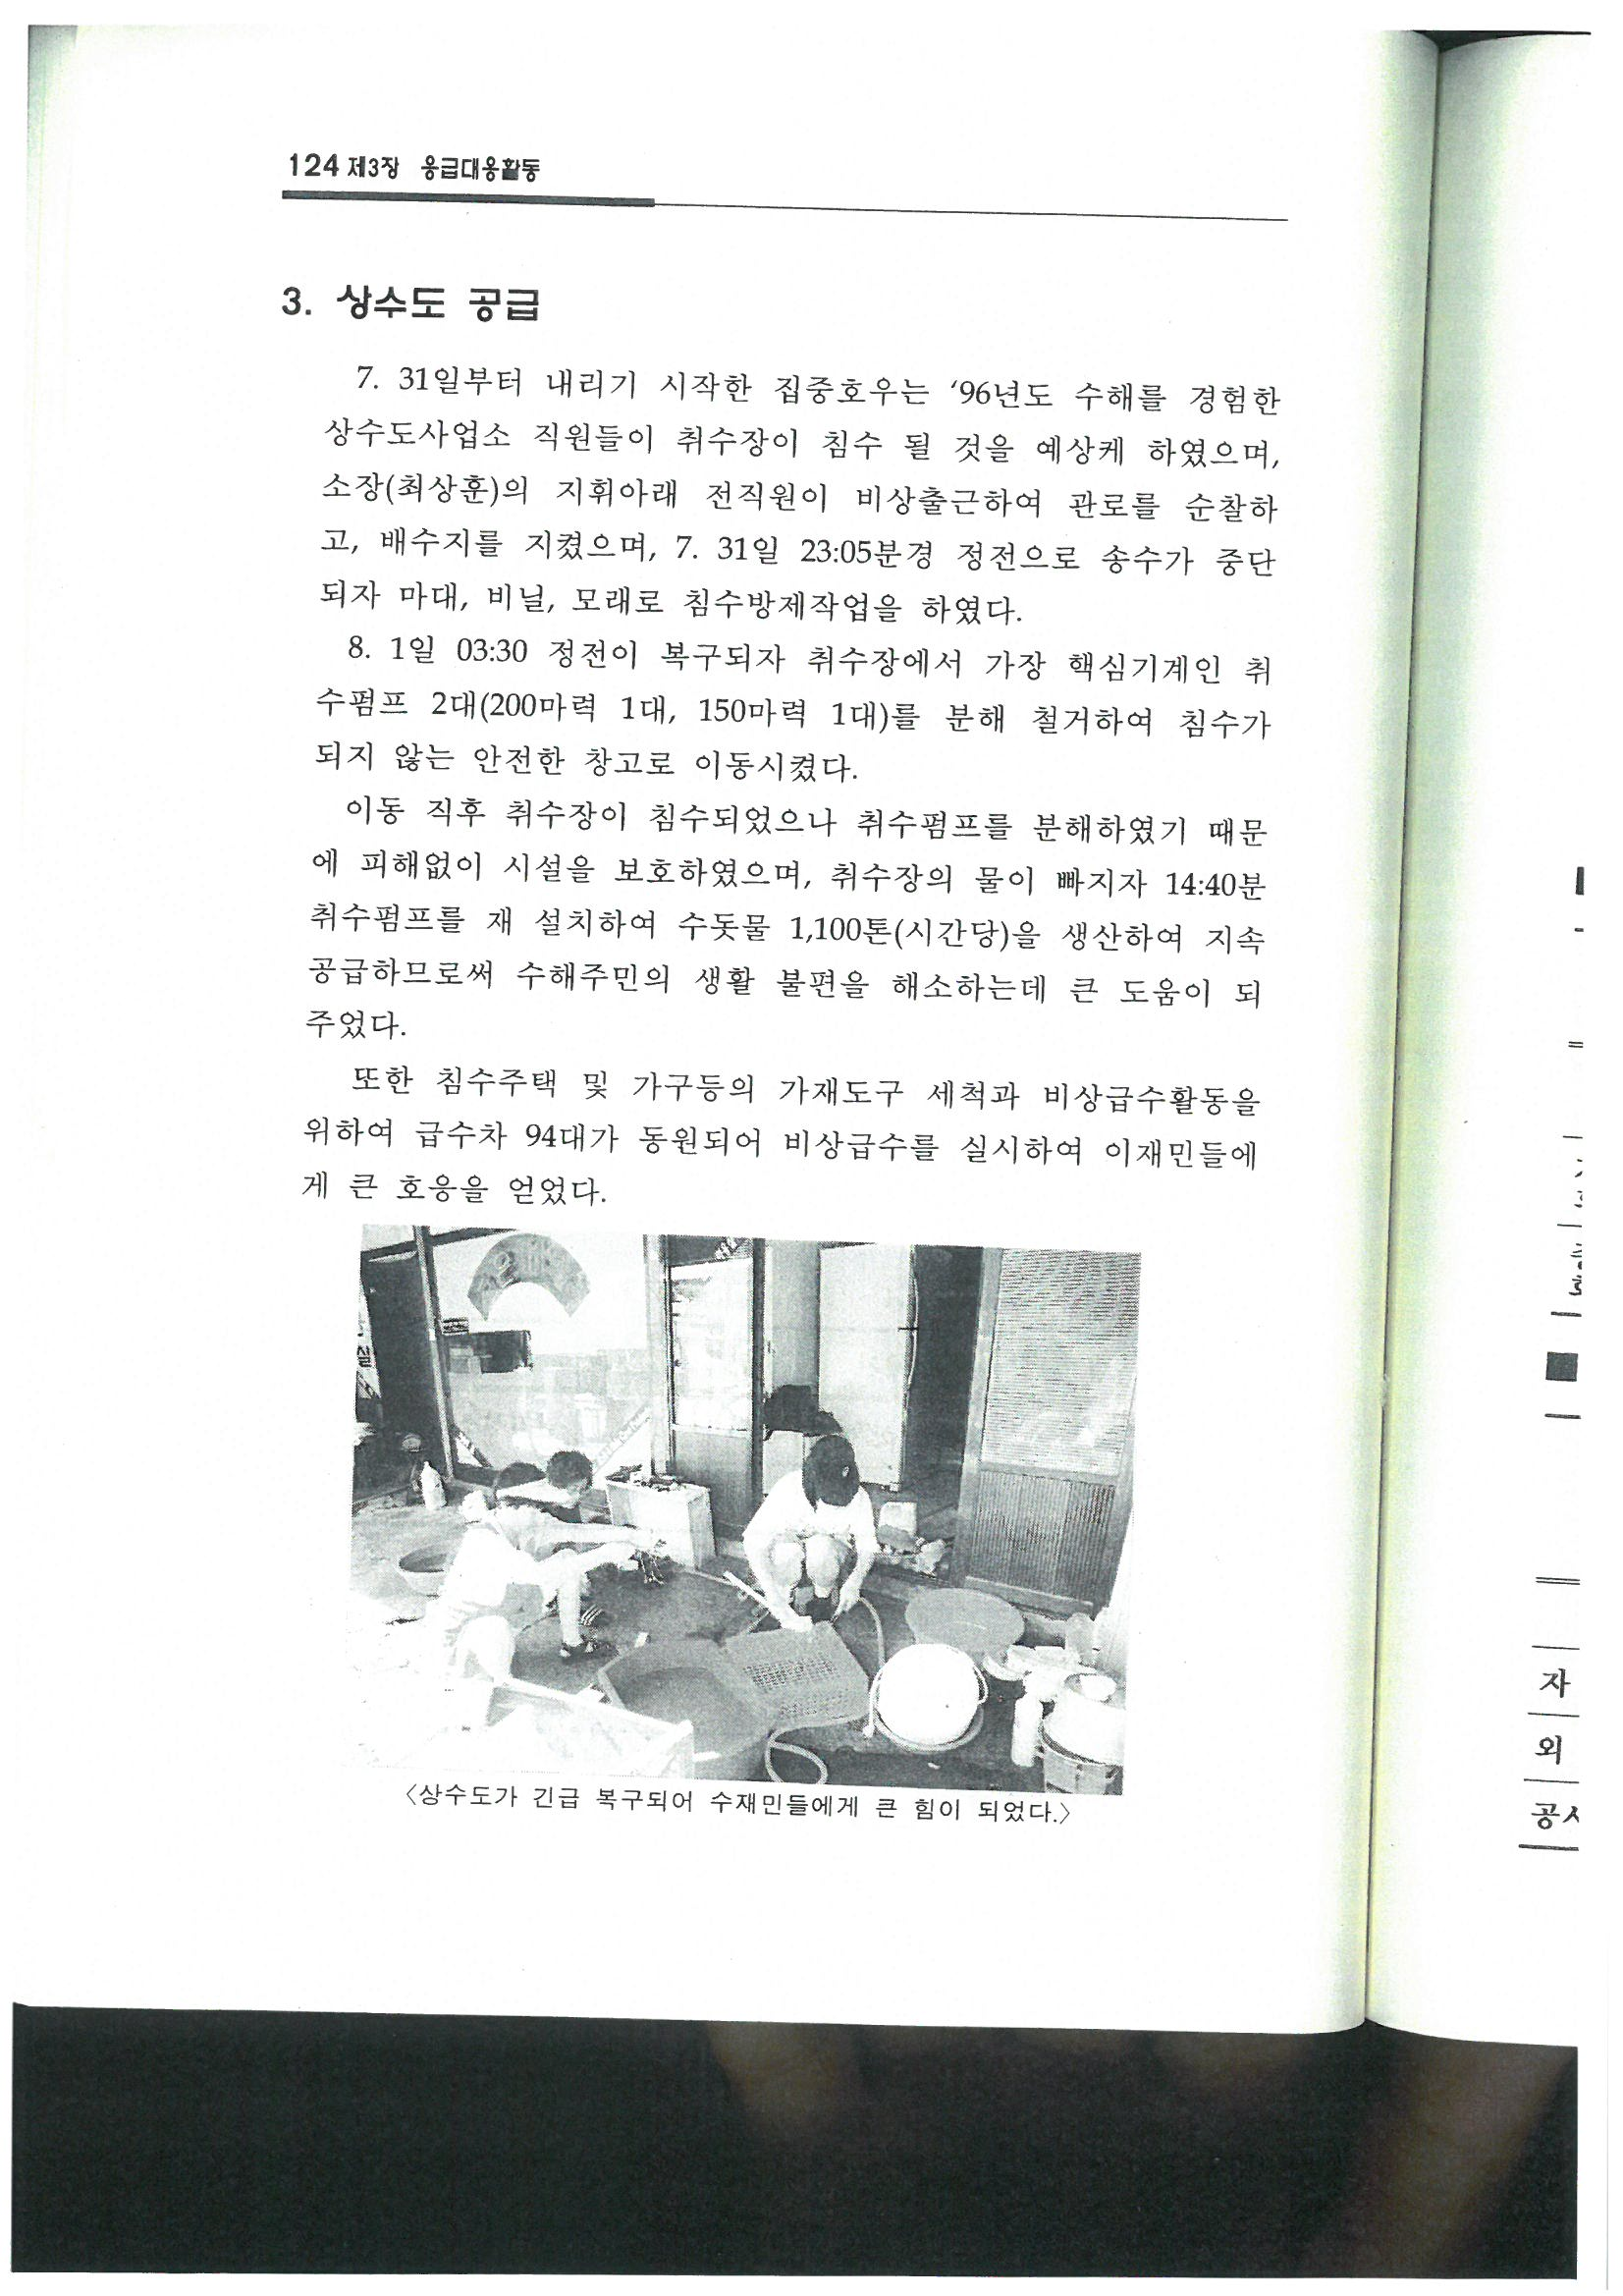
\includegraphics[scale=0.5]{DBs/pic/006.jpg}\\
\caption{99년 수해백서 발췌}
\end{figure}


\subsection{상수도 정수약품 투입방식 자동화}	

일반직으로 전직하고 맑은물관리사업소에서 근무를 하다보니 우선 시스템을 이해하여야 하는데, 상수도를 공급하기 위환 순서는 우선 취수장에서 원수를 끌어올리면 중량물인 부유물은 침사지라고 하는 곳에 우선 가라앉히고, 급속혼화기에서 물의 흐름을 급속히 요동시키며, 그 곳에 응집제를 투입하면 응집침전지에서 가벼운 부유물을 큰 덩어리로 만들어 침전시키고, 모래 속을 통과하는 여과지를 거쳐, 흔히 수돗물 하면 냄새나는 것을 느끼게 하는 지구상에서 가장 강한 살균제(염소소독)을 거쳐 읍내리 산 위에 있는 배수지로 올려 각 가정으로 공급이 되게 하는 것입니다.

그런데 가장 핵심인 정수약품 투입방식을 보니 대수제어방식(펌프가동 댓수에 따라 투입량 결정)으로 하고 있는데, 수질의 상태에 따른 투입량 결정 등은 담당자의 임의판단에 의하여 조절하고 있었습니다.

그래서 그 방식을 바꾸고자 취수유량계는 설치가 되어 있으니 약품펌프에서 유출되는 양을 측정하는 약품유량계를 설치하고, 많은 시행착오를 거쳐 수질상태에 의한 약품투입비율(PPM)×취수량(㎥/min)=약품투입량(ℓ/m)이라는 수식을 가지고 자동제어프로그램 기사에게 부탁하여 투입방식을 수정해 수질안정성을 확보하였습니다.


\begin{figure}[t]
▣ 메모보고\\
\tabulinesep=1.2mm
\begin{tabu} to \linewidth {|X[1,c]|X[4,c]|}
\hline
제목 & 약품투입 자동운전 \\ \hline
보고자 & 허호강 / 맑은물관리사업소 / 지방공업주사보 / 031-839-2860 \\ \hline
보고일 & 2009.08.17 15:21:47 \\ \hline
\multicolumn{2}{|c|}{
원수 수질변동에 따른 수질사고 사전예방을 위하여
}\\
\multicolumn{2}{|c|}{
응집제 투입방식을 자동으로 개선 운전하였으면 함 
}\\ \hline
첨부 & 약품투입방식.xls[17KB] \\ \hline
\end{tabu}
\caption{약품투입 자동운전 제안 메모 발췌(2009년)}
\end{figure}

\section{2000년대}

\subsection{55㎏에서 65㎏으로}
고등학교 시절부터 괴롭혀온 위장병은 드디어 현대 의약품의 발전에 힘입어 해방 2002년도 1년 사이에 55㎏이었던 몸무게가 65㎏로 허리둘레 32인치가 남아돌던 것이 36인치가 빵빵하도록 불어나고, 아침을 반 공기 먹으면서 이것이 점심시간까지 소화가 될까 걱정하면서 식사하던 것이 이제는 식사하고 조금 지나면 시장기를 느끼는 행복(배고파지는 것이 그리 큰 행복인지 몰랐음)을 느끼고, 건강검진에서 혈액검사를 하면 영양공급이 안 되서 그런지 마냥 맑음으로 나오던 것이 봄에 발이 시려서 혈액검사를 하니 이제는 영양이 넘쳐서 고지혈증에다가 콜레스테롤 등 수치가 5배가 넘도록 변화가 되고, 소요산 하백운대를 절반도 못 올라가고 하산하던 체력이 한라산, 지리산, 설악산, 태백산을 등정할 정도로 좋아져 혈당 및 고지혈로부터 건강을 지키기 위하여 꾸준히 운동을 하여 이제는 모든 컨디션이 정상으로 돌아 왔습니다.

\subsection{고등학교 중퇴에서 대학교 졸업}

친구 중에 한명도 고등학교 중퇴자가 있었는데 ``나 서울 가는데 같이 갈래?''하기에 따라 갔더니 청와대 뒤에 있는 경복방송통신 고등학교로 가더니 ``나 여기 올해 졸업하는데 너도 여기서 고등학교 과정을 마치라''고 권유를 하여 그래 `나도 공부는 좀 해야지'하고 2학년 과정으로 편입학하고 매월 2주씩 일요일 9시부터 5시까지 수업, 무난히 마치고 나서 대학을 어디로 진학할까 하고 생각해보니 연천군 주변에 학교도 없고, 그리고 정작 배우고 싶은 공과대학도 없어, 아내가 먼저 방송통신대학교 일본학과 과정을 배우고 있어 나도 그거나 해야겠다하고 시작한 것이 그래도 어찌어찌 그 과정까지는 수료를 했는데, 그 당시부터는 안구 건조증에 의한 안구염증이 눈동자를 조이는 듯 아파서 책을 보는 것이 힘들어져 공부는 거기까지만 하고 건강관리에 모든 것을 집중하고 있습니다.

\subsection{연천군 상수관망도 작성}

맑은물관리사업소 시설급수팀에서 근무하며 퇴근 후 직원 몇 명이 석양주 한 잔 하다가 우리 상수도관로에 대한 관망도가 있으면 좋겠다는 이야기를 하여, 그 현황을 찾아보니 2004년도에 캐드 프로그램으로 작성된 관망도가 있었는데 활용도 못하고 있어 그것을 기초로 하여 관망도 작성을 위하여 서울시 상수도사업본부 및 남양주시 수도과를 견학 2009년 7월에 `상수도 유수율 제고 및 효율적 재산관리를 위한 상수관망도 일제정비 및 GIS추진계획'이라는 계획을 수립하고 추진하면서 기존 작성되었던 캐드파일을 연천군 도로명지도 연속지적도로 옮기는 작업을 하는 중에, 추경예산에 반영할 노트북 구입비계상과정에 직원간의 마찰이 있자 문제 있는 직원은 놔두고 의욕적으로 사업을 추진하던 사람을 요금계로 보내버리고 내가 추진하던 관망도 사업은 그대로 묻혀버리게 되었습니다.

그 사건으로 가슴속에 분노가 차있으니 몸도 같이 아파져서, 정신과 치료를 받고 마음의 안정을 가지고 요금팀에서 나름대로 체납요금관리 상하수도 사용료 현실화를 위한 요금인상 등 일을 찾아하던 중. 인사이동으로 새로운 소장이 부임하여 그동안에 있었던 것을 이야기 하고 관망도 사업은 추진하는 것이 좋겠다고 의견을 제시하니 바로 예산에 반영하고 사업을 추진하여 주셨습니다.

마음이 아프면 몸도 같이 아파진다는 것을 뼈저리게 느끼고, 모든 일을 추진함에 있어 우선 모든 상황은 공유를 하고 다 같이 이해를 했을 때 진행해야지 내가 아무리 좋은 일을 옳은 방향으로 추진한다 하더라도 다 같이 동참의지가 없으면 독불장군이 되고 그것은 옳지 않다는 것을 가슴속 깊이 체감 하였습니다. 
\begin{figure}
▣ 메모보고

\tabulinesep=1.2mm
\begin{tabu} to \linewidth{|X[1,c]|X[4,c]|}
\hline
제목 & 활기찬 맑은물 관리사업소를 만들어 갑시다 \\ \hline
보고자 & 허호강 / 맑은물관리사업소 / 지방공업주사보 / 031-839-2860 \\ \hline
보고일 & 2009.08.27 05:33:20 \\ \hline
\end{tabu}
\begin{tabu} to \linewidth{|X[j]|}

활기찬 맑은물관리사업소를 만들기 위한 제안입니다.

제안에 앞서 우선 요즈음의 제가 느낀 사항에 대한 말씀을 먼저  드리겠습니다. 맑은물 생산에 주력하기 위하여는 우선 근무체계가 우선 개선되어야 하는데 모든 직원이 알고 있는데도 담당자는 움직이질 않고 있고, 사업을 추진하기 위하여는 주무부서에서 적극 지원이 되어야 하는데 좀 미흡한 것 같습니다.

제가 맑은물관리사업소에 온지도 10개월이 넘었습니다. 처음에 와서 스테플러가 없어서 구입을 요청한지 근 7\textasciitilde8개월은 되어서 구입이 되었고(문구정도는 필요한 직원이 언제든지 사용할 수 있도록 하는것이 필요함), 당직실의 침구 개선요청은 아직도 처리되지 않고 있으며, 샤워실의 비누가 떨어지기 일수고,  전화 교환기의 냉각팬 소음때문에 옮기는 것이 좋겠다는 의견도 현재까지 무시되고 있으며, 선곡리 유량계실의 압력과다로 문제가 발생되어 외부 압력계를 설치하는것이 좋겠다는 의견도 업체의 가능하다는 판단이 서 있는 현재도 품의서가 돌아가지 않고 있고, 또한 응집제 투입방식에 대한 개선안으로 엑셀의 함수 마법사를 이용하여 수량과 탁도에 의한 자동투입방식을 제시하였는데 않되는 방향으로 설명을 들어야 했습니다.

더구나 제가 요즘 역점적으로 추진하고 있는 관망도 GIS사업에 사업계획서를 7월에 작성 협조부서까지 다 결재를 받고 부군수, 군수 결재를 부탁하였는데 8월 25일 사무실에서 소동이 있은 후에야 결재를 받았고, 추경예산에 현장확인용 노트북을 계상토록 시설급수분야 예산편성 담당자에게 의견을 제시하였는데 우선 누락되었고(제가 시설직 선배였어도 그랬을지?) 그것을 가지고 정수물품 승인을 받아야 한다는 물품담당자에게 부군수까지 결재받은서류를 복사해 주면서 언성이 좀 커지자 관리담당은 "내 앞에서 뭐하는거야. 군수결재 받아와"하면서 소리지르고, 10년이나 후배인 회계담당까지 "안 도와 준게 뭐가 있어요"하고 같이 큰소리 치고.

너무나 분한 나머지 연가내고 집에가서 혼자있으니 눈물이 쏟아지고 안먹던 술도 마시고 잔뜩 마시고, 맑은물 생산을 위하여는 항상 좋은 의견이 적극 반영되는 그런 사무실을 만들어 갔으면 좋겠다고 생각합니다. 붙임 문서는 제가 설움을 당하면서 까지 추진하고 있던 GIS 사업 추진계획서 입니다.
\end{tabu}
\tabulinesep=1.2mm
\begin{tabu}  to \linewidth {|X[1,c]|X[4,c]|}
\hline
첨부 & 상수관망도 일제정비 및 GIS 추진계획.hwp[873KB] \\ \hline
\end{tabu}

\caption{상수관망도 일제정비 및 GIS추진계획 메모 발췌}
\end{figure}
\newpage

\begin{figure}[t]
\centering 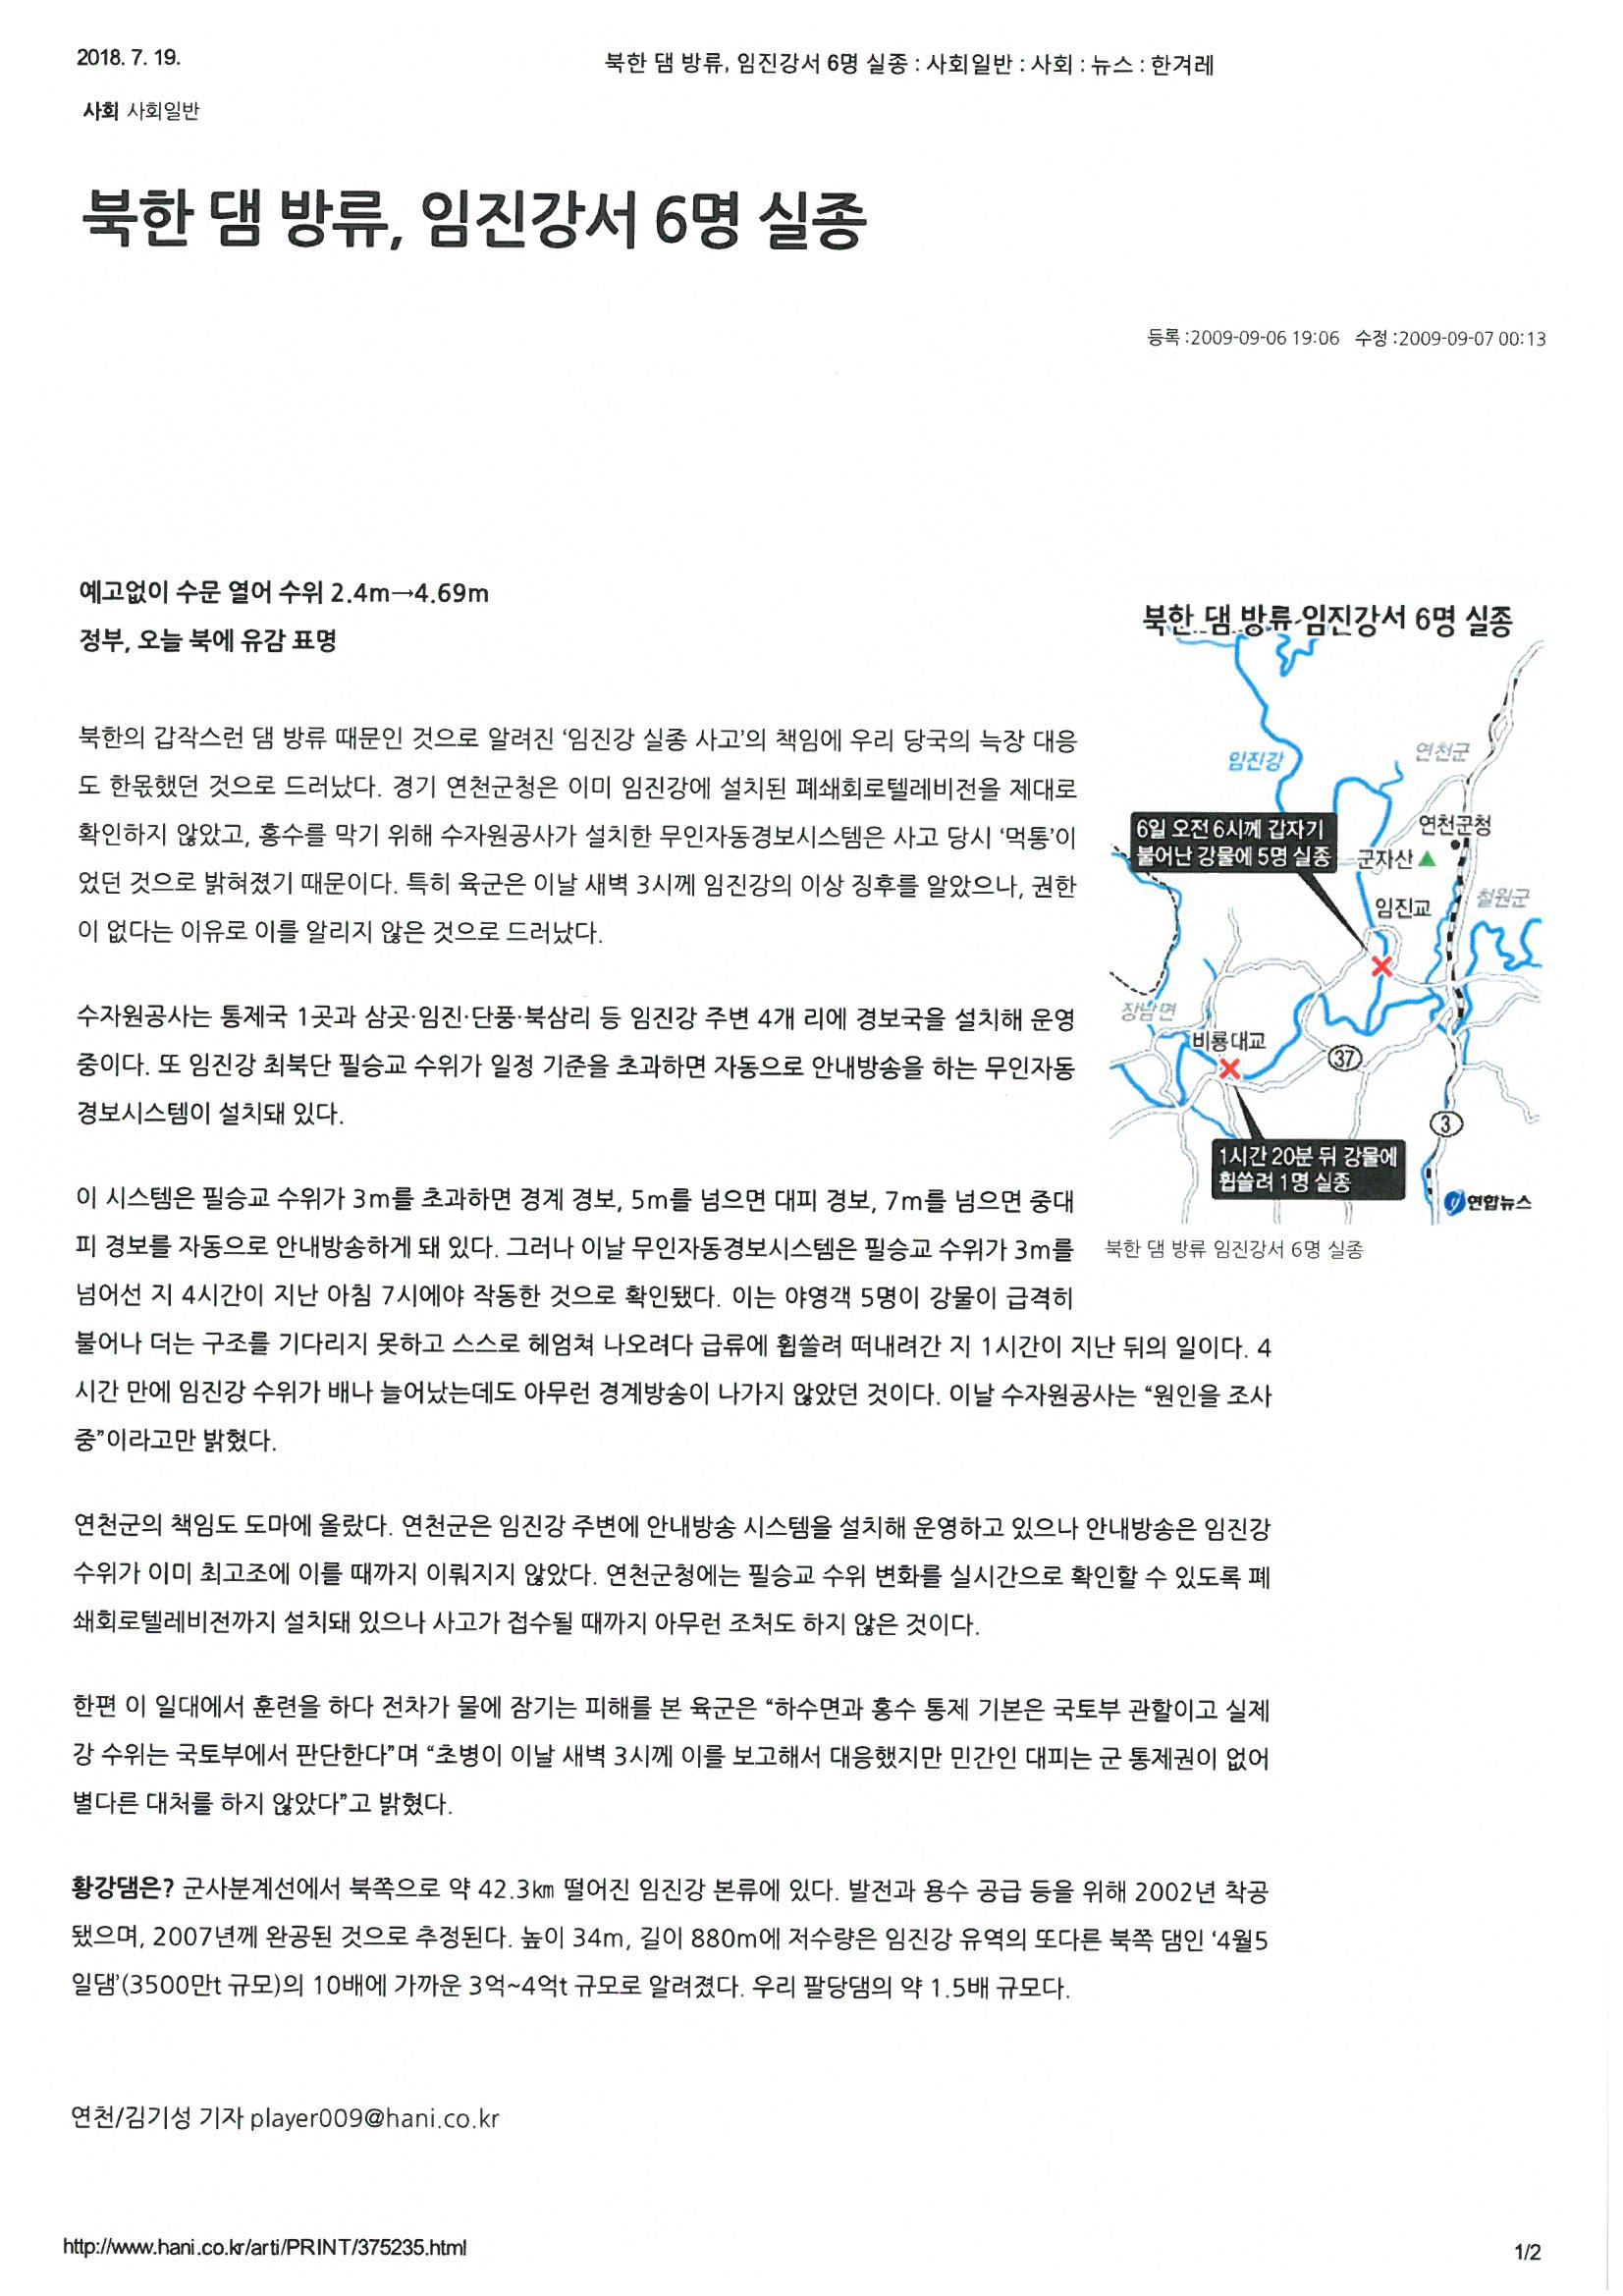
\includegraphics[scale=.5]{DBs/pic/007.jpg}
\caption{2009년 9월 9일 신문기사 발췌}
\end{figure}



\subsection{북한 댐 방류, 임진강서 6명 실종}

2009년 9월 6일 북한에 있는 황강댐(군사분계선에서 42㎞ 상류에 2007년에 준공된 댐)에서 갑작스러운 방류로 인해 `임진강 실종사고'로 6명이 실종되는 사건이 발생하였습니다. 

이 사건으로 우리 군에서는 당직하였던 직원이 구속까지 되었었는데, 그 당시에는 임진강 댐을 건설 중이여서 수자원공사에서 자동으로 안내방송을 하는 무인자동 경보시스템이 설치하고 관리하고 있었는데, 사고가 발생되자 수자원공사에서는 우선 사망자에 대한 보상처리를 하고 법률전문가들이 적극 나서서 보상금에 대한 것을 연천군에 구상금으로 청구하여 회수하여 가져갔습니다. 그런데 연천군에서는 당직매뉴얼에도 없는 상황에 직원이 구속되는 상황이 되는데도 사건초기부터 적극적인 변호사 조력 없이 당사자 혼자서 당하는 것을 보았습니다.

나중에 `연천읍 도시가스공급사업'에서 다시 언급하겠지만, 공무원이 정당한 공무를 수행하면서 사법기관의 수사를 받게 되는 등의 사건이 발생하면 초기부터 적극적인 법률자문가의 도움을 받을 수 있게 지원을 하는 것이 담당자의 사기진작과 아울러 업무회피를 사전에 예방하는 것이 필요하였던 것 같습니다. 


\subsection{민원인 때문에 훈계조치}

요금팀에서 체납되는 상하수도요금을 정리하던 중 상수도요금은 조례에서 정한대로 일정기간 체납되면 정수조치하면 되는데, 지하수를 사용하며 발생되는 하수도사용료는 별도의 제재조치가 없어 한번 체납이 되면 자진하여 납부할 때 까지는 계속 체납상태가 되고 있었습니다. 체납해소를 위하여 토지소유자를 조사하여 지방세체납처분의 예의 절차에 따라 압류처분까지 마쳤는데 압류예고까지 아무 반응이 없던 소유자(나와 친족관계라 알고 있는 사이임)가 당사자가 아닌 부군수 및 기감실장한테 욕을 하면서 압류처분을 풀어놓으라고 하여 내가 민원인한테 전화를 하면 응대를 하지 않고 다시 부군수나 기감실장한테 욕을 하며 생떼를 부리고, 그런 일이 있고 나서 웬 훈계장이 도달, 참으로 채권보전을 위한 행정행위에 대한 부당한 민원인의 요구에 담당자가 훈계처분을 받아야 하는 지 참으로 황당한 일도 있었습니다.

\section{2010년대}

\subsection{연천읍 도시가스 공급사업}

맑은물관리사업소에서 지역경제과로 발령을 받고 녹색성장팀으로 배치되어 보니 당면 현안사항이 군수공약사항이자 연천읍 주민 숙원사업인 `연천읍 도시가스공급사업'을 담당자로 업무를 진행하게 되었습니다.

도시가스 사업자인 (주)대륜E\&S와 수많은 회의와 함께 관련부서 협의를 걸쳐 협약서 초안까지 마련하여 2013년 02월 13일 도시가스 사업자와 협약을 체결하고, 주민설명회 등을 거쳐 전곡읍 은대리 미소육화로부터 연천읍 현가리 고향손두부 칼국수까지 3년간에 걸쳐 본 사업을 추진하게 되었습니다.

사업은 순조롭게 진행되던 중, 2014년 04월 28일 일부 지방지에서 관련규정은 확인도 하지 않고 도시가스관 되메움제로 재활용골재를 사용하는 것을 부실시공이라는 기사를 게재하였으나 충분히 해명을 하였는데, 연천경찰서에서는 이것을 사건화시켜 무려 4년 간이나 수사를 하여 18명을 피의자로 검찰에 송치하였는데, 그 서류 양이 방대하여 검찰에서 서류를 검토하는데만 무려 6개월, 그리고 서류상으로는 피의자, 그러나 검찰수사관한테 진술할 때는 참고인적인 대우를 받으면서 검사와는 단 한차례 전화통화(업무추진을 왜 그리하였는지에 대하여 묻기에 업무를 효율적으로 처리하기 위하여 그리하였습니다.)로 마무리되어, 2017년 07월 19일 무려 4년 3개월에 걸친 수사와 피의자 18명에 대한 수사가 종결되어 현재 연천읍에는(물론 일부이기는 하지만) 도시가스를 사용하고자 하는 가정에서는 별 문제없이 도시가스를 공급받고 있습니다.

평상시 업무추진 과정에서도 의도적으로 잘못한 것은 결과에 따라 당연히 처분을 받아야 하는 것이라는 신념을 가지고 업무에 임하였는데, 아무도 추진해보지 않은 업무를 추진하다 보니 오류는 있겠지만, 이것은 형사적인 사건보다는 행정적인 사건으로 봐야 하는 것을 수사대상자를 무조건 범죄자로 만들려는 일제 강점기 순사보다도 더한 수사행태에 참으로 아직도 민중의 지팡이라기 보다는 자기 자신의 영달을 위한 권력을 휘두르는 것에 참으로 아연실색하지 않을 수 없었습니다.

\subsection{지하수법 관련}

공직에 입문 후 26년 만에 처음으로 팀장이라는 보직을 부여받아 3번째로 맑은물관리사업소로 발령, 업무담당자가 아닌 보조자로서 보니 가장 초보적인 민원업무인 지하수개발·이용신고가 업자들의 무질서한 행위 때문에 민원인이 많은 어려움을 겪고 있는 것을 보게 되었습니다.

절차대로는 아니지만 그래도 업자는 민원인이 불편하지 않도록 행정행위를 대행하여야 하는데, 무조건 지하수를 굴착 정상적인 취수가 되면 대금만 받고 관련서류 절차를 이행하지 않고, 취수량이 부족하면 계약금도 돌려주지 않은 채 연락이 두절되는 등 민원인이 건축허가 및 농업보조금 등 관련 인허가에서 여러 가지로 불편을 겪는 것을 경험하여, 이후로는 담당자에게 질서를 위반하는 업자는 과감히 관련법령에 의하여 처분토록 하여 4건에 3명의 지하수개발업자가 2천만원의 과태료를 물도록 하여 이후 지하수관련 질서를 확립하여 민원인의 불편을 최소화 하였습니다.

또한 「지하수법」 및 「하수도법」에 의하면 지하수 수질검사 및 정화조 청소의무 등 주기적으로 이행하도록 규정되어 있어 이를 이행하지 않으면 관련규정에 의하여 과태료를 처분토록 되어있으나, 이것은 전국 시군이 공통으로 이행되지 못하는 규정으로서, 지하수 및 정화조를 사용하는 자는 도시지역이 아닌 대부분 농촌에서도 외딴지역으로서 농촌빈집이 늘어나고 있는 시점에 사용하지도 않는 시설물에 대한 의무를 가지고 과연 과태료처분이 가능한지, 만일 과태료를 처분을 하면 처분대상자를 명확히 하여야 하는데, 이러한 것은 또한 소유권변동 및 사용자에 대한 등록의무도 없는 상태에서 이를 처분하면 행정효율은 있는 것인지, 그런데도 각 시·군 종합감사에서는 이것보라는 듯이 지적사항으로 나오고 있어 2017.02.20일 민생현장의 애로사항이 있는 사항에 대한 규제개선을 팀원들과 의논하여 요구한 바 있으나, 아직 관련규정 개정은 요원한 것 같습니다.  공무원은 법을 준수하여야 하는 의무가 있으나 지키지 못하는 법령 때문에 제약이 되어 업무를 적극적으로 하지 못하는 것은 결국 국민을 잠재적인 범법자로 만들고, 또한 담당자의 업무 의지를 위축시키는 결과가 될 것입니다. 

\subsection{환경기초시설 관련}

연천군에서 가장 혐오시설에서 근무하는 환경기초시설(하수도, 분뇨, 가축분뇨) 관리대행 업체에 근무하는 직원들은 관리자(소장 및 중요기술자) 이외에는 전부 연천군 주민으로서 열악한 환경에서 근무하는 것에 대하여 격려하고, 주변 민가에서도 그동안의 악취 및 수집운반차량 통행으로 인한 피해의식에 대하여 대화분위기를 조성하고자 `환경기초시설 근무자 단합대회 및 체육행사'를 2016.04.22(금) 남계리 환경사업소에서 시행, 군수님의 격려가 있을 예정이었으나, 갑작스러운 OBS인터뷰로 인하여 부군수님이 대신 격려하시고 소요물품은 전체 맑은물관리사업소의 부서업무 추진비로 결재하여 행사를 무사히 마무리하였습니다.

이후 연천군 자체감사에서 농협에서 구매한 물품 중에 주류가 있는데 이것은 예산집행기준에 위배된다고 하여 확인서를 작성하여 주었는데, 감사결과 통보에서 이것을 회수조치하였는데 회수는 혜택을 받은 사람이 납부하는 것이 당연할 것인데, 참석자 전원이 혜택을 받았으면 다 같이 나누어 내야 하는 것인지 아니면 기획을 잘 못한 담당자가 내야 하는지, 또한 마트에서 구입한 영수증이 총괄영수증이 아닌 내역영수증을 첨부한 담당자가 내야 하는지(그렇다면 앞으로 업무추진비로 결재하는 모든 것은 내역영수증을 첨부하여 주류가 포함되지 않은 것을 확인해야 할 것임) 그러면 그런 것은 의도한 잘못이 아닌 단순한 업무착오면 지도를 하는 것이 아닌가 하는 생각이 들면서, 혐오시설근무자의 사기앙양과 아울러 주변지역주민을 위로한다는 것이 담당자에게 그런 부담을 주면 누가 그동안에 없었던 일에 대하여 창의적으로 업무를 할 것인가는 다같이 생각해야할 앞으로의 숙제가 될 것입니다.

신서면 전방지역에 있는 군부대가 자체적으로 사용하던 오수처리시설에서 공공하수도로 유입시키기 위하여 2006년도에 5사단에서 연천군의 허가를 받아서 공사를 한 것이 제가 부임한 2015년도에도 준공검사가 안돼서 원인을 살펴보니, 부실시공으로 인한 하천수 유입에 따른 불명수 유입과  아울러 지뢰밭으로 관로가 매설되어 점검도 할 수 없이 시공된 상태에서 신서하수종말처리시설로 유입되어 수질관리에 막대한 지장을 초래하고 있어 우선은 행정적인 잘못은 나중에 조치하더라도 수질관리 안정성 확보가 우선이라 이를 해소하고자 군부대 담당자들과 수차례에 걸친 회의와 공문을 주고받으며 추진하였으나, 군부대에서 발생하는 생활하수는 공공하수도로 들어가고 있으니 미온적으로 대응하고 있고, 이를 적극적으로 추진하는 과정에서 다른 팀과의 의견충돌이 있어 소장실에서 회의를 하던 중 몇 년이나 후배인 팀장이 자기와 의견이 다르다고 욕하고 싸우자고 대들어, 이런 조직사회에서 내가 있어야 하나 하고 생각하며 인사팀에 명예퇴직 신청서를 바로 제출하니 주변에서 만류하며 좀 쉬다오라고 하여 일주일동안 휴가를 내고 마음을 가다듬어 출근을 하니, 당사자는 사과 한마디 없고 같이 근무하는 친구가 술 한 잔하고 싶다고 전하였으나 본인이 진정으로 사과하지 않으면 아무 의미가 없어 그 이후로는 서로 마주치지 않고 있습니다.

지역경제과에서 근무할 당시 산업통상자원부에서 시행하는 `지역에너지 절약사업'을 각 부서에 시달을 하고 맑은물관리사업소에서 환경관련 업무를 하다 보니 에너지도 절약되면서 수처리효율도 좋은 공법이 있다는 제안을 받아 살펴보니, 수중에 산소공급을 미세한 공기방울로 만들어 접촉효율을 높이면서 전력사용량 1,944㎾/일을 사용하는 기계설비를 1,010㎾/일로 줄여 8년을 운영하면 투자비용이 절감되는 기술적, 경제적, 사회적 측면에서 상당한 효과가 있는 사업인지라 곧바로 다음해에 사업신청을 하여 추진하게 되었습니다.

이외에도 저는 태생이 가만히 있지 못하는 습성이 있어 글로서는 다 표현을 못하겠고, 그동안에 제가 겪었던 것 중 일부만 서술한 것은 어공에서 늘공으로 이제 다시 전업농으로 돌아가면서 이러이러한 것들은 세상이 변한 만큼 변화가 되지 않아야 하겠나 하는 심정으로 이 글을 남기고자 한 것입니다.

\chapter{마무리하며}

\section{퇴직 후 전업농을 선택한 이유}

공무원 임용 전까지 농업에 종사한 적도 있지만, 환경보호과에서 근무할 때 하수도 소독시설관련 유럽에 견학하면서 유럽 등 서양국가에서는 농업을 소득이 적은 산업으로 보는 것이 아닌 생명을 다루는 직업으로 존중받고 있고 또한 고소득도 보장이 되는 사업이라는 것을 보고 느끼는 바도 있었고, 그 동안에 몸에 익혀온 조그마한 상하수도 관련 수처리에 대한 지식도 접목시켜 이것저것 해보고 싶었는데, 정년을 몇 년 앞둔 2015년도 퇴직 후의 미래를 생각하면서 농지가 한 필지라도 있었으면 좋겠다고 생각하며 여유 있는 시간에 생전 경험도 없는 경매검색을 하다 보니, 한눈에 딱 들어오는 물건이 있었는데 이 땅이 내 땅이다 싶어 무조건 경매기일에 참석 조금 넉넉하게 입찰에 응하니 낙찰, 더욱 농업에 전념할 수 있는 계기가 마련되었고 농업(農業)의 농(農)자의 글자를 풀어보면 곡(曲노래)자와 진(辰별)자가 합하여 `별을 노래하는 직업'이라고 하겠습니다.

농업은 물론 많은 노동력을 필요로 하는 고된 직업인 것은 틀림없으나. 옛날의 농사방식에 비하면 농업기계화와 아울러 고도의 농약기술의 발전으로 많은 노동력 절감이 이루어 졌으니 옛날방식으로는 경쟁력을 가질 수가 없는 것이 현실입니다.

제가 방황의 시절(표 1, 연간총소득 산출내역)에 기술하였던 바와 같이 세월이 변하여 많은 농산물의 가격변동도 많았고, 또한 주요 소득작물도 많이 변화하였습니다. 식량작물 위주에서 고소득을 위한 각종 새로운 품목들이 대거 재배되고, 또한 농가당 경작면적이 몇 천평 단위에서 몇 만평 단위로 늘어나 예전방식으로 농사를 경영하다보면 가족이 생계를 영위하는 것이 불가능한 것은 사실입니다.

우선 3년 동안의 영농경험을 말씀드리면, 2016년도에 구입한 농지 1000평(3299㎡)에 첫 벼농사를 경작하니 농기계사용료 등 198만원 영농비용에 쌀 판매 수입 252만원에 순수익 52만원, 2017년도에 밭으로 변경하여 검은콩(서리태)를 경작하여 본 결과 100만원 영농비에 콩판매수익 301만원에 순수익 211만원, 2018년도 200만원 영농비에 판매수익 900만원 예상에 순수익 700만원은 확보될 것으로 예상됩니다. 이 경우는 영농이 전업이 아닌 직장생활을 하면서 틈틈이 영농한 사항으로, 전업농이 될 경우 규모늘 늘리고 품목을 다변화하면 충분히 경쟁력이 있을 것으로 보았습니다. 물론 농업소득은 하늘이 결정하여 주는 것이고 농업인은 최대한의 소득을 보기 위한 노력만 하면 될 것입니다.

그동안 많은 분들이 이제 퇴직하면 무엇을 할 것인가 물어들 보시곤 하셨는데, 제 입장은 확고부동하게 농업을 할 것이라고(농사라고하면 일만하고 소득이 없는 것으로 비쳐짐)하면 왜 힘든 일을 하냐고 평생을 일을 했으면 편안히 연금으로 여행이나 하면서 생활이나 하지 왜 생고생을 하려고 하느냐고 말씀들을 하시면 저는 그것을 설득하기가 곤란해 입을 다물곤 했습니다. 

농업 작업은 예전에는 수제농기구로만 일을 할 때 하루종일 같은 일만 반복하는 매우 힘든 일이라 각종 근육통 및 관절염 등 직업병의 원인이었지만, 지금은 농기계를 효율적으로 이용하고 농약과 비료를 적정량을 사용하면 노동력 절감과 영농효율을 높여 고소득도 창출 할 수 있을 것으로 생각합니다. 

\begin{figure}[b]
\centering \subfloat[][벌레의 공격을 받은 배추가]{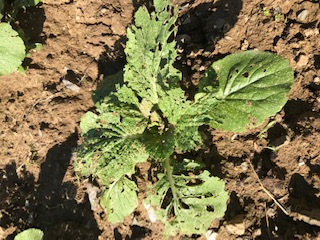
\includegraphics[scale=.45]{DBs/pic/008.jpg}}
\qquad
\subfloat[][효과적인 방제로 이렇게 됩니다.]{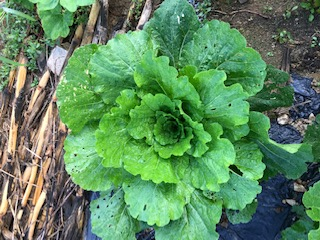
\includegraphics[scale=.45]{DBs/pic/009.jpg}}
\end{figure}
           

또한 농약에 대한 제 소견을 말씀드리고자 하면, 인간의 수명을 획기적으로 늘리게 된 것이 농약개발과 함께 이루어지지 않았나 생각합니다(순전히 개인의 생각임). 동식물은 자기방어를 위하여 병해충의 공격을 받으면 자기를 방어하기 위한 물질을 생산해 낼 것입니다.(상처가 난 나무주변은 두툼하게 되어있으며, 사람도 상처가 나거나 세균의 공격을 받으면 진물이 나고 딱지가 앉는 등 저항물질을 생산함) 아래 사진과 같이 벌레의 공격을 받은 배추는 자기를 지키기 위한 물질을 만드느라 초록색을 잃어버리는데, 벌레의 공격을 멈춰주면 탐스러운 녹색의 색깔을 가지게 되는 것 같습니다.

저는 평소의 소신이 모든 먹거리에는 약과 독이 함께하고 있어 아무리 몸에 해로운 물질이라도 적정량일 때에는 약이 될 수 있지만 아무리 몸에 좋은 음식이라도 조금이라도 과하면 곧 몸을 공격하는 독이 될 수 있다고 생각하고 있습니다. 농약과 비료의 적정한 사용으로 우리는 지금 식량위기에서 벗어날 수 있었고, 또한 풍성한 먹거리가 생산될 수 있었다고 생각합니다.  농약은 독극물은 분명하나 모든 국가에서는 `농약 잔류허용기준제도(PLS)가 있어 이 기준을 정확히 지키면 건강한 농작물 먹거리가 될 것입니다.

또한 주로 해산물의 경우 자연산과 양식에 대한 구별에 대하여도 저는 천적과 병해충으로부터 보호받는 양식이 더욱더 우수한 먹거리로 보는데, 물론 양식업자가 과도한 항생물질을 사용하지 않는다는 조건이 있습니다. 마당에 뛰어다니는 닭과 알맞은 크기의 운동장을 갖춘 닭장에서 기른 닭 중 더 맛있고 영양가가 풍부한 쪽은 아마 후자일 것입니다.

2008년도에 온 나라를 뒤 흔드는 광우병사태를 보면서 사람들이 선동되면 국가의 존망을 위태롭게 만드는구나 하고 절실히 느꼈습니다. 식품위생기준 등의 먹거리에 대한 제도가 우수한 선진국에서 생산되는 소고기를 단지 동물성사료로 사육된 소중에서 일부 발생되는, 더구나 30개월 월령이 지나지 않으면 전혀 문제없는 수입소고기를 화면 가득히 바둥거리며 일어서지 못하는 병든 소를 계속 광우병에 걸려있는 소로 오인하도록 방영하여 국민을 호도하는 것을 목격하면서도, 우리나라에서도 소는 많이 키우고 키우다 보면 각종 질병으로 병들은 소도 발생되고 병든 소가 발생되면 그 마을의 수의사가 진단하고 관련부서에 신고하여 죽어있으면 부패하지 않도록 배를 갈라서 도축장으로 보내서 처리하곤 하였습니다.

연천지역도 많은 목장들이 있고 저도 80년도에 소를 키운 바가 있어서 일련의 이런 사항을 다 알고 있는데, 그저 TV에서 광우병소가 들어와서 큰일이 났다고 국민들을 호도하여도 일부 학자들 이외에는 말하는 사람들이 없었습니다.

\section{후배공직자들에게 바라고 싶은 것들}

제가 공직생활을 하면서 그동안 이런 것들은 이제는 변화해야 하지 않나하고 평상시 생각하였던 것들을 모아 봤습니다. 단순히 우리가 변화하는 것이 아닌 국민 모두의 생각이 바뀌어야 하는 것이 아닐까 싶어 이글로 남겨 보고자 합니다.

\subsection{농업정책에 대하여}

농업은 1970년대 까지는 우리나라의 기반산업으로 자리를 잡고 있었으나 급격한 사회변화와 농업기계화로 인하여 각자 소득확보를 위하여 새로운 작목들이 많이 들어오고 있습니다.

최근에 사과대추, 아로니아, 블루베리 등등 그리고 기후변화로 인한 주산지 변동 그러나 우리나라의 면적은 좁고 소비자도 한정 돼있는데 이것이 수익성이 높다고 생각되면 너도나도 재배하면 처음에 시작한 농가는 소득이 되는 반면 막차를 탄 농가는 그야말로 패가망신하기가 십상입니다. 

그래서 국가단위의 농산물에 대하여 총량제 라는 것을 해봤으면 하는 생각을 해 보았습니다. 이러한 정책은 국가단위에서 해야 할 것이나 농정제도 개선 같은 의견제출 계기가 있으면 제시하여 농가들이 한번 씩은 생각하여야 할 문제일 것 같습니다. 

원리는 간단할 것입니다. 전국적으로 재배하는 주요농산물에 대한 연간 총 수요량에 대하여 지역별 및 품목별로 농가들의 경작면적 및 생산량을 할당하여 신청토록 하고 신청 받은 작물에 대하여는 자연재해 등 최소 소득에 대하여는 국가에서 소득을 보장하여 주고 추가로 발생된 생산량에 대하여는 농가의 소득이 되도록 하는 것입니다. 여기에 동참하지 않는 농가는 수익과 손실에 대하여 본인이 책임지도록 하면 국가농산물 총 생산량을 효과 있게 조절할 수 있을 것입니다.

\subsection{교육문제에 대하여}

우리나라의 교육문제는 어떻게 변화 하는 것이 중요 한 것이 아니라 부모가 자녀에게 바라는 바를 어떻게 바꾸어 나가는 것이 좋은가라고 생각합니다.

점수에 따라 정해져 가는 자기의 진로가 아닌 자기가 하고자 하는 바를 이끌어 나가는 것이 진정한 교육이라고 생각합니다.

작금의 고위공직자 및 정치인들의 행태를 보면 인성이 갖추어지지 아니한 고득점의 점수에 의하여 벼슬이 정하여 지다보니 국민은 안중에도 없이 정권쟁탈과 눈치 보기에 급급하여 정치적인 혼란을 일으키는 것은 나이외의 사람이 보이지 않기 때문일 것입니다. 우리 자녀가 무엇을 공부하고 싶은 가가 아니라, ``너는 공부를 잘 해서 이걸 해야 되''라고 하는 부모의 이기심이 공교육은 불신을 받고, 사교육비로 인한 지출이 가계부에 상당한 부담과 국가적인 문제를 일으키게 되고 국가에서 수립하는 교육정책은 이해관계에 따라 호불호가 너무 심하게 갈리고 있습니다. 아무리 좋은 정책도 좋은 국민이 아니면 실행될 수가 없을 것입니다. 난세에 영웅이 난다고 하였는데, 내가 편안할 때에는 누가 무엇을 잘해줘도 고마움이 없는데 불편할 때 조금만 도와줘도 엄청나게 고마운 것하고 같은 이치이겠지요. 

중국에는 요순시대라는 신화가 있었습니다. 자세한 것들은 검색 하여 보시고 나라님이 무엇을 하는지 모르는 평안한 시대로 알려져 있습니다. 

우리는 지금 나라가 무엇을 하는지 무슨 일이 벌어지고 있는지 또한 너무 많이 알고 있으니 이런 시대가 과연 국민이 편안한 시대인지는 생각 좀 해 봐야 할 문제입니다.

우리나라의 근현대사에서는 영웅은 없고 역적만 있는 국가가 되어가고 있다는 생각이 듭니다. 지나간 역사를 가지고 진실이 무엇인지 보다는 어느 것이 정당성인지가 우선시 되는 그래서 그것의 해석이 다른 쪽은 무조건 부정하고 그것이 또한 정의라고 생각하며 그것을 꼭 교육과정에 포함시키려는 의도가 국론을 분열시키는 역할을 하고 있습니다.

역사적인 인물들이 많은 우리나라에서 근현대에 들어서는 위인전에 올라갈 사람이 없는 것은 무엇을 이야기 하는 것일까요. 고조선시대의 낙랑공주와 호동왕자부터 을지문덕, 김유신, 김춘추, 태조왕건, 강감찬, 세종대왕, 이순신 이외에도 수많은 위인전을 읽고 교육받고 자라왔는데 지금의 잣대로 따지면 하나의 잘못이 드러나 곧 능지처참되어야 할 인물이 될 것은 자명합니다.

공무원으로 재직하면서 북한, 일본, 중국, 서유럽, 동유럽 미국 러시아 등 견학과 개인여행의 기회가 있어 가서 느낀 점은 저는 그곳의 역사적인 배경과 주민의 의식 같은 것을 주로 관심을 가지고 다녀왔습니다.

우리가 교육받은 대로 하면 러시아는 엉큼한 곰이 도사리고 있고, 일본은 뻐드렁니에 호시탐탐 남의 영토나 노리고 있고, 중국은 곡괭이와 망치로 중무장한 인해전술을 주 무기로 하는 무지몽매한 못사는 나라로, 북한은 괴뢰군이라고 하여 빈곤과 악마의 이미지로 교과서와 홍보물에 가득하였던 것이 방문하여 보니 모든 선입견은 사라지고 국민들 자체는 순수하고 오로지 정치지도자들의 의도에 의하여 길들여져 있다는 것을 느껴졌습니다.

올해 초 자유여행으로 오키나와를 여행하면서 국제거리를 구경하다 시장 안에 들어섰다가 골목길이 보여 이 길로 가면 지름길이 되겠다고 생각하고 조금 들어가 보니 길이 좁아져 그냥 돌아서 나오니까 그걸 보고 있던 현지인이 따라오더니 갈 수 있다고 하면서 골목 끝까지 데려다 주었습니다. 이러한 친절이 몸에 밴 국민을 우리는 혐한시위를 하고 군비경쟁이나 하는 나라로 우리나라 언론이나 정치권에서는 홍보를 하는데 현지의 국민들은 검소하고도 순수하며 친절하였습니다. 우리 언론에서 말하는 전쟁을 위한 국가로 가고자 하는 것은 일부 정치지도자들의 의도적인 문제 뿐 인걸로 보였었습니다.

made in china는 우리나라에서는 불량품의 대명사로 인식되고 있는데 중국에 가서 첫 번째 느낀 것이 화장실의 화장지가 우리나라 그 어느 것보다 고급스럽고, 공산품 역시 좋은 것들이 가득하였고, 농수산식물 또한 좋은 것은 내수로 소비하고 잔여생산물은 수출한다고 하였습니다. 그러면 불량품의 대명사는 어찌 된 것인가, 이는 우리나라의 수입상이 수익을 최대한으로 올리기 위하여 저질품을 가져다 판매하는 것에 기인하는 것이라고 판단하였습니다. 일본에서는 식자재를 수입하기 위 하여는 사전 조건이나 위생기준이 엄격하여 예전에 우리나라에서 수입을 해 갈 때도 그 기준에 맞아야 수입을 해가고, 그것은 다른 국가에도 아마 마찬가지 일 것입니다. 그런데 우리나라의 수입상들은 수익성을 우선시 하다보니 저렴한 인건비의 저질품만 가져다 파니 중국산은 무조건 나쁘다는 인식을 가지게 되었던 것 같습니다. 

이 외에도 다른 국가에 대한 평가보다는 왜 우리는 이런 선입견을 가지고 있는가를 보면 어려서부터 교육에 각 국가가 왜 이러한 이미지를 가지게 되었는지부터 알려주고 여건에 따라 다른 나라를 침략하고 침략당하고 그런 역사적 문화적인 배경도 같이 알려주면 이러한 왜곡은 사라지고 국가들 간의 신뢰가 더 생겨날 것입니다.

일본이 임진왜란을 거쳐 메이지유신 이전의 아주 빈곤한 시절의 정치지도자 중 이시다바이간(石田 梅岩)(1685∼1744)이라는 정치지도자가 있었는데 (제업 즉 수행[諸業卽修行], 혹은 제업 즉 수업[諸業卽修業])이라는 석문심학(石文心學)을 주창 하였는데 ``일이 곧 수행이요, 일이 곧 수업''이라는 학문을 펼쳐 일본제품이 세계제일의 명품이 되도록 하고, 경제부흥을 일으키는 계기가 되어 경제대국이 되는 근간을 이루어준 것입니다. 이 석문심학의 교육에 기인하여 온 국민이 일치단결하여 ``일하는 것이 곧 도를 닦는다''고 하면서 국가발전을 이루었습니다.

중국도 수많은 내란(혁명)을 겪으면서 내란이 한번 나면 몇천만명 씩은 기본으로 죽어나가는 역사적인 배경이 있습니다. 진나라를 시작으로 하여 왕족이 바뀔 때 마다 우리나라 인구 보다 더 많은 백성이 한꺼번에 목숨을 잃게 되는 사건이 비일비재 하였습니다.

겨우 60년 전만 하여도 정권을 놓치기 싫은 국가지도자가 국민을 선동하여 홍위병을 앞세워 문화대혁명이라는 사태를 일으켜 3만 4천명이나 죽었으며 또한 공산주의 국가인 현재의 중국은 중국식 사회주의라는 표명 아래 서방국가 보다 더한 자본주의가 팽배해져가고 있어, 등소평의 개혁개방에 힘입어 처음으로 북경에서 올림픽이 열리는데 올림픽경기장 건설을 할 때 말이 끄는 마차와 인력으로 공사하는 모습이 매스컴에 나왔고, 저임금노동자를 이용하기 위하여 우리나라의 노동집약적 산업과 공해유발산업들이 중국에 대거 진출하였는데 이제는 중국의 인건비도 상당히 높아졌고 우주선을 쏘아 올리는 국가가 되어 지금은 동남아로 다시 빠져 나가고 있는 실정으로 이미 중국은 자본주의가 상당히 팽배하여 초일류기업이 그득한 나라가 되었습니다.

이외의 다른 나라들도 나름대로 훌륭한 역사와 사회제도를 가지고 있는데 우리는 학생들에게 제대로 된 사실보다는 우리와 적대관계와 이해관계에 대해서만 가르치고 있는 것 같습니다. 일본군의 위안부 문제만 하더라도 구한말 당파싸움으로 국력을 피폐하게 만들어 다른나라가 침략을 하여도 무방비로 당하게 한 우리나라 정치지도자가 잘못한 것이지, 이웃나라가 약해 질대로 약해져 침략을 하여도 대항하지 못하는 오판을 하도록 하여 침략한 것에 대하여 사과하라고 하는 것이 맞는 것인가, 제가 초등학교 때 선생님이 하신 말씀 중 ``남의 물건을 훔쳐간 사람 보다 훔쳐갈 마음을 가지도록 한 것이 더 나쁜 사람''이라고 하시는 말씀을 들은 적이 있습니다. 

정치적인 목적을 달성하기 위하여 위안부할머니들을 이용하여 더 그들의 가슴을 아프게 하지 말고 과거를 교훈삼아 나라발전을 위하여 무엇이 더 합리적인 것인가는 서로 많은 논의를 하여야 할 것 같습니다. 진보와 보수, 자본주의 공산주의 이러한 이념성을 가진 편 가르기보다는 사업가는 사업에서 최대한의 이익을 창출하여 고급일자리를 양산하고, 또한 그 수익만큼 세금을 납부하고 그에 따르는 복지사업 등으로 사회에 헌신하고, 기초생활이 어려운 취약계층은 최소한의 생활보장을 국가에서 책임지는 제도를 만들 수 있도록 학생들에게 가르쳐야 할 것입니다.

제가 퇴직을 준비하고 있는 요즘 사립유치원 비리라고 국정감사에서 거론되고 언론에서 계속 떠들어 대고 있는데 이것이 과연 비리인가 아니면 정치적인 의도인가가 저한테는 의심되고 있습니다.

사립유치원은 「유아교육법」 제8조(유치원의 설립 등) 제2항에 의하여 교육감에게 `설립 인가 신고'를 하고 인가된 유치원에서는 「같은 법」제25조(유치원의 원비)제1항의 규정에 의한 원비를 받게 되어있습니다. 또한 제26조(비용의 부담 등)제2항의 규정에 의하여 대통령령으로 정하는 바에 의하여 국고의 일부를 지원을 할 수 있도록 되어 있습니다. 그러면 원비를 받아 자기사업을 하는 사립유치원인데 일부 지원을 받았다고 해도 그것이 국가의 소유가 아닌데 명품빽 이라던가 성인용품구입 등을 가지고 논란이 되는 것을 보면서 지도점검은 공무원이 하는 것이고, 또한 잘못이 있으면 국가나 담당공무원이 책임지고 잘못한 부분에 대하여 처분을 하여야 하는 것인데 사유재산인 유치원에 국공립회계프로그램 도입을 달성하기 위하여 사립유치원 설립 운영자를 부도덕한 사람들로 매도하고 국민의 공분이 동원되게끔 하는 것은 아닌가 생각합니다. 맑고 순수하게 놀면서 친구들과 선생님 그리고 부모님과의 인과관계를 소중하게 배워 나가야하는 유치원생들이 원장님한테 ``원장님이 나쁜 짓을 하셨다면서요''. 하고 질문을 할 정도로 교육을 담당하는 분들한테 너무 정치적인 논리를 가지는 것은 참으로 뭐라 할 말이 없습니다.

저는 인터넷 강의를 즐겨 봅니다. 스타강사 중에 김미경 강사의 강의를 의미 있게 들었습니다. 그 중 일부 강의내용 일부입니다.
\begin{quote}
김미경 ``운동이 재능입니까? 아닙니까?, 

방청객 ``재능입니다.''

김미경 ``음악이 재능입니까? 아닙니까?''

방청객 ``재능입니다.''

김미경 ``공부가 재능입니까? 아닙니까?''

방청객 ``?????''
\end{quote}
김미경 ``공부도 재능입니다. 부모들 본인들이 공부를 잘해서 의사나 박사 법조인이 되지 왜 자녀들한테 시키는 거죠? 그렇게 자녀들한테 공부를 시키는 것 보다는 본인이 하시면 되는 거죠, 허리 튼튼하지 공부도 해 봤지 본인이 하면 되지 왜 자녀들한테 시키는 거죠?''

저 또한 교육은 자율에 의하여 하는 것으로 생각하고 있던 터에 김미경 강사의 강의를 듣고 나서 더욱 확고한 믿음을 가지고 본인들의 의사를 존중하여 원하는 진로를 결정할 수 있도록 환경조성에 더욱 치중하게 되었습니다.

\section{우리 군 행정에 대하여}

제가 공무원으로서 재직 중에 느꼈던 사항에 대하여 그 당시에 표현을 하지 못한 것은 현직에 있으면서 의견을 제시하면 불평불만을 나타내는 것으로 보여질 수 있어, 퇴직을 준비하면서 동료와 후배들께서 참고될 만한 것인지는 한 번 고려하여 봤으면 하면서 몇 자 적어봅니다. 

현재의 세대는 급격한 변화에 의하여 단순화 돼있던 공무원의 직종이 다양화되어 소수직렬들이 많이 생겨나고 있습니다. 그 소수직렬들은 무엇을 덜 한 것이 아니고 그 분야에 더 필요한 능력을 가진 자원인 것입니다. 그러기 때문에 꼭 필요한 인원만 임용하는 것 보다는 정수의 2배수 내지는 3배수 까지 임용하여 한 분야만 계속 근무하는 것이 아닌 다양한 부서를 경험하게 하여 그 경험을 바탕으로 전문직의 기술력과 우리 군 실태를 제대로 파악하여 경력이 쌓이면 꼭 필요한 인재들이 될 것입니다.

지방의 기초자치단체는 정부의 축소판으로서 각 부처에서 관장하는 업무를 겪어 보면 여러 분야에 적용 가능한 부분들이 많을 것입니다. 그리고 진급은 당사자들이 신경 쓰지 않고 자기 직분에 최선을 다하면 충분한 보상을 받는 시스템이 되어야 할 것입니다. 진급을 한 사람의 정당성을 이야기하는 것 보다는 경력과 연륜이 되었는데도 진급을 못하는 당사자에게 진급에서 누락된 이유가 설명이 되어야 할 것입니다. 물론 뜬소문이라고 치부할 수도 있겠지만, 누구누구는 누구에게 부탁하고, 누구와 연결이 되어있고, 이런 소문이 현실화 될 때 자기노력에 많은 노력을 한 공직자들은 실망감이 클 뿐 아니라 자기능력개발에 전념하지 않음으로써 조직사회 발전에도 큰 저해요소가 될 것입니다.

공무원이 업무를 추진하다 보면 늘 하던 일은 사전에 검토된 사항이라 그대로만 하면 법에 저촉될 일이 없지만, 처음으로 추진하는 일들은 계획단계부터 충분히 검토하고 자문하고 하지만 그래도 법령 어딘가에는 저촉되는 사항이 있습니다. 법(法)이라는 글자를 풀어보면 물 수(
\includegraphics[scale=0.045]{DBs/pic/011})자와 갈 거(去)자가 합쳐진 글자로서 물이 흘러가는 것을 법이라고 할 수 있습니다. 공무원은 물이 잘 흘러가도록 치수관리를 하는 것이 중요한 일이라고 하겠습니다. 괜히 물길을 막고 다른 방향으로 틀어대고 하면 물이 요동을 치거나 고였던 물이 터지면 큰 피해를 당하게 되는 것입니다. 그래서 법은 사람을 위해서 만든 것이기 때문에 법을 제정할 당시의 제정취지를 이해하고 업무를 추진하는 것이 중요하다고 할 것입니다.

저는 담당자로서 근무할 때도 그렇지만 팀장이 되어서도 직원들과 업무를 하면서 글자 하나하나에 의미를 부여하지 말고 법이 만들어 질 때 왜 만들어졌는지를 먼저 생각하라고 하였습니다. 어떠한 행위를 하고 나서 감사 내지는 점검을 받을 때 의도적인 잘못이 아니고 단순한 착오정도면 업무지도로 충분한 것을 글자하나하나에 의미를 부여해 지적이 되고 처분을 받는 다면 모든 공무원이 창의적인 업무보다는 있는 그대로만 하려고 하는 이른바 사회 병폐라고 하는 복지부동이 만연할 수뿐이 없습니다.

제가 친구들과의 저녁식사 시간에 ``넌 어느 부서에서 근무 해보고 싶냐?''하고 묻길래 감사팀에 가서 한 번 일해보고 싶다고 했더니 누구랑 안 좋은 일 있냐고 하길래 그게 아니고 업무의 형태를 한 번 바꾸어 보고 싶다고 한 적이 있었습니다. 

올 여름 고양시에서 행정안전부 감사관의 갑질 행태가 뉴스에 보도된 적이 있었습니다. 그 감사관은 우리 군 에서도 감사를 진행 한 적이 있었고 저도 환경시설팀에 있을 때 업무와 관련하여 감사장에 갔었는데, 수사권도 없는 감사관이 무슨 중죄인 심문하듯이 질문 하길래 우선 다 듣고 나오다가 감사팀 직원에게 ``저놈은 어떤 놈인데 감사관이 공무원을 죄인취급 하냐''고 물어보니 행정안정부 조사팀장인가 하는데 그냥 참으시라고 하고 다음에 또 갈일이 있으면 아주 녹음해서 해당 장관한테 이메일로라도 보낼 까 했는데 다시 부르는 일이 없어서 그냥 지나갔습니다. 

감사관의 입장에서는 지방공무원이 무조건 잘못하는 게 보이는지 몰라도, 잘못한 것이 있으면 확인서 받고 문서로서 처분하면 되는 것을 윽박지르고 조그마한 잘못도 크게 만들어 가려고 하는 행태를 보이는 것이었습니다. 물론 국가의 안위를 위하여는 공무원이 철저하게 질서를 지켜야 하겠지만 조그마한 법 위반사항은 없어야겠지요.

지방자치단체 ``정부합동평가''라는 것이 있습니다. 정부에서 목표점을 정해놓고 순위를 매기는 것으로, 좋은 의미를 가진 평가목록도 있지만 불필요한 것도 목록에 있어 지방자치제도에 전혀 어긋나는 것으로 이야기 하려는 것입니다. 

우선 간단하게 장애인 생산품, 녹색제품, 여성기업인 생산품 등 국가에서 보호해야 할 대상이 있어 구매순위를 정하는 것은 지원 대상 기업의 자생력을 떨어뜨려 시장에서의 경쟁력을 잃게 될 것입니다. 공익광고 중에 ``진정한 후원은 후원을 멈추게 하는 것입니다.''라는 내용이 있습니다. 각종 사업을 추진 할 때 제품은 가장 좋게, 공사품질은 우수하게 하려고 할 때 걸림돌이 되고 있는 현실인 것입니다. 보호해야 할 단체에게는 구매를 도와주는 것이 아니라 제품을 향상시켜 시장에서 살아남게 하는 방향으로 해야 할 것이고, 시장개척도 본인들의 몫일 것입니다.

그리고 마지막으로 한가지 제가 맑은물관리사업소에서 있으면서 상수도 신설급수 체계를 바꾸어 보면 어떻겠냐고 담당자와 담당팀장 및 팀장회의 때와 감사기간 중에도 이야기 해 보았습니다. 상수도신설급수신청은 신청인이 신청서를 작성하여 제출하면
\begin{center}
대상지 현지 출장 ⇒ 출장복명 및 설계, 급수승인 및 고지서 발부 ⇒ 신설 급수공사비 및 시설분담금 납부 ⇒ 신설공사 발주 ⇒ 준공 및 급수 
\end{center}
이런 절차를 급수공사대행업체가 접수를 받으면
\begin{center}
신청인이 급수공사대행업체에 신청서 접수 ⇒ 담당자는 현지출장 후 승인 ⇒ 대행업체 공사 ⇒ 준공 및 급수
\end{center}
 하는 절차로 도시가스 공급 및 하수도 배수설비 신청접수 절차를 준용하고자 한 것입니다. 기대효과로는, 공사비는 맑은물관리사업소 고시가격 내에서 업체와 민원인과 계약하고, 시설분담금도 대행업체에서 대리납부토록 하면 공사업체와 민원인과의 계약관계로 서비스 향상과 아울러 공사품질도 좋아질 것으로 보이며, 또한 담당자의 업무량은 현저히 줄어들 것입니다. 퇴직인사를 하면서 이와 같은 거론을 한 것은, 이런 것이 향후 업무개선에 도움이 되었으면 하는 바램에서 적어 보았습니다.

\section{마치며}

이제 저는 전문농업인으로서의 길을 가려고 합니다. 저에게 약 1년 전부터 많은 지인들이 향후 진로에 대하여 물어봅니다. 그러면 저는 농사가 아닌 농업을 경영할 거라고 하면 10명 중 9명은 ``왜 그 힘든 일을 하려고 하냐''하면서 말리시는데, 물론 저를 걱정 해 주시는 고마운 마음이지만 저는 오히려 잘 해보라고 격려를 바라는 쪽이었습니다.

농업에 대한 오해를 좀 풀려면, 농사일은 하루 종일 같은 일만 반복하여 신체를 망가뜨리는 직업병의 근원으로 알고 있지만, 요즘 현실은 우리가 출장 다니면서 들판의 농지를 보면 종일 일하는 사람은 없습니다. 농기계와 농약 그리고 비료로 계획영농이 가능하기 때문에 우리 부모님세대와는 달리 뼈가 뒤틀리거나 근육이 망가지는 그런 일은 없습니다.

물론 힘은 들지요. 그렇지만 제가 4\textasciitilde5년 전에 공복혈당이 140이 넘었었는데 요즘은 정상치보다 더 낮은 120이하로 조절되었고 허리둘레와 몸무게 또한 지극히 정상입니다. 나이가 들면 들수록 몸을 편히 두면 안된다고 생각 하는게 저의 철칙입니다. 일하면서 건강도 갖고 소득도 있고, 거기에다가 누구든지 귀농귀촌은 생각하는 사람이 있으면 도움이 되려고 합니다. 또한 농촌의 고령화로 어려움을 겪고 있는 농민들과 함께 있으면서 조금이라도 저의 공무원 경험이 도움이 된다고 하면 도움을 드리도록 노력하겠습니다.

그리고 저의 아들들도 최대한 저의 계획에 어느 정도 호응을 하여 저 혼자 고집하여 하는 것은 아닙니다. 일은 시키지 않고 경험을 가지도록 하는 것이 저의 생각입니다. 저의 아내도 22살에 시집와서 저와 같이 공무원생활을 하고 있어 농업경험이 전혀 없지만 저의 농업경영에도 적극 동참하고 있습니다. 물론 가끔 일에 대하여 의견차이로 티격태격 하지만 그래도 같이 하고는 있습니다.

저는 일은 시키지 않습니다. 일을 시키면 분명히 의견충돌이 있고 이는 곧 다툼이 되겠지요. 하고싶은 일을 하다 보면 어떤 것이 더 옳은가 의견이 통일되면 효율이 더 높아지겠지요. 목공예가 해보고 싶다고 하는데 농막에 작업장용 하우스를 지어놓고 공구를 하나 둘 장만하다 보니 이제는 만들고 싶은 것 있으면 제도해서 톱질하고 연마를 거쳐 못질하면 제품이 하나 씩 되겠지요.(물론 멍석깔아 놓으면 마음이 틀려지겠지만)

이제 저는 출퇴근에 얽매이지 않고 형식에도 제약받지 않는 내가 하고 싶은 일 해야 할 일을 찾아서 하려고 합니다. 제가 농지를 구입하고 나서부터 지금까지의 영농내용을 블로그에 작성해 놓아보았습니다.
\begin{center}
https://blog.naver.com/hhkangg
\end{center}
개방된 블로그로서 눈팅하고 가셔도 됩니다. 

전자결재의 권한이 곧 끝나가게 되어 서둘러 글을 쓰다 보니 두서없이 내용도 뒤죽박죽인 것 같습니다. 여러분들과 함께 한 시간은 저에게 참으로 멋진 행복한 순간으로 간직될 것입니다. 글을 쓰는 것이 1이고 교정하는 것이 9인데 저에게 준비된 시간이 없어 글을 늘어놓는 것으로 최종 마무리 하겠습니다. 연천군청 공무원 가족 여러분 건강하시고 행복하십시오.

{\flushright
2018년 10월 18일 16:20}\\
{\flushright지방공업주사 허호강 드림}
\end{document}


   \setstocksize{266mm}{196mm}
     \settrimmedsize{260mm}{190mm}{*}
 \setlength\trimtop{\stockheight}
 \addtolength\trimtop{-\paperheight}
 \setlength\trimedge{\stockwidth}
 \addtolength\trimedge{-\paperwidth}
 \settrims{.5\trimtop}{.5\trimedge}
 
 
   \settypeblocksize{200mm}{120mm}{*}
   \setlrmargins{*}{*}{1.5}
   \setulmargins{*}{*}{1.0}
   
   
   \setheadfoot{16pt}{30pt}
   \setheaderspaces{*}{18pt}{*}
   \setmarginnotes{10pt}{100pt}{10pt}
